\documentclass[
    bachelor,
    blackurls,
    titleikn
]{mthesis}

\setcounter{secnumdepth}{3}
\setcounter{tocdepth}{3}

\usepackage{adjustbox}
\usepackage{booktabs}
\usepackage{float}
\usepackage{graphicx}
\usepackage{makecell}
\usepackage{pdflscape}
\usepackage{sidecap}


\graphicspath{ {./sections/images/} }

%%%%%%%%%%%%%%%%%%%%%%%%%%%%%%%%%%%%%%%%%%%%%%%%%%%%%%%%%%%%%%%%%%%
% Параметры класса документа

%---------
% тип ВКР
%---------
% bachelor  - бакалаврская диссертация
% master    - магистерская диссертация

%-------------
% гиперссылки
%-------------
% blackurls - ссылки на литературу, таблицы, рисунки, формулы и т.п.
%             не выделяются цветом (используется для ч/б печати)
% colurls   - цветные ссылки (для распространения пояснительной записки 
%             в электронном виде)

%-----------------------------
% оформление титульного листа
%-----------------------------
% titlestd  - согласно методическим указаниям
% titleikn  - согласно требованиям ИКН


%%%%%%%%%%%%%%%%%%%%%%%%%%%%%%%%%%%%%%%%%%%%%%%%%%%%%%%%%%%%%%%%%%%%
% Здесь следует размещать допольнительные пакеты и команды. Следующие 
% пакеты уже загружены в стилевой файл: geometry, amssymb, mathtools, 
% ifthen, cmap, textcomp, babel, upgreek, indentfirst, xcolor, calc, 
% tabularray, icomma, ulem, soulutf8, tikz, hyperref, graphicx, 
% caption, subcaption, pdfpages, aliascnt, totalcount, totcount, 
% totpages, placeins, enumitem, biblatex, fancyvrb, listings



%%%%%%%%%%%%%%%%%%%%%%%%%%%%%%%%%%%%%%%%%%%%%%%%%%%%%%%%%%%%%%%%%%%%
% Информация для заполнения титульного листа и задания на ВКР

% ФИО студента
\AuthorShortName{Бутаков Б.И.}
\AuthorFullName{Бутаков Богдан Игоревич} % полностью
\AuthorFullNameGen{Бутакову Богдану Игоревичу} % полностью в родительном падеже
% Номер группы
\AuthorGroup{БИВТ-22-16}

% Тема работы
\ThesisTitle{Оценка стоимости ремонтных работ в автосервисе с применением методов машинного обучения}

% Научный руководитель
\SupervisorShort{Агабубаев А.Т.}
\SupervisorFull{Агабубаев Аслан Такабудинович}
\SupervisorDegree{Старший преподаватель кафедры АСУ}

% Нормоконтроль
\GOSTComplianceReviewer{Смирнов С.С.}
% Проверка на заимствования
\PlagiarismChecker{Кузнецов К.К.}

% Название кафедры, ФИО зав. кафедрой
\DeptShort{АСУ}
\DeptFull{АВТОМАТИЗИРОВАННЫХ СИСТЕМ УПРАВЛЕНИЯ}
\DeptHead{Темкин И.О.}

% Название института, ФИО директора
\InstShort{ИТКН}
\InstFull{ИНФОРМАЦИОННЫХ ТЕХНОЛОГИЙ И КОМПЬЮТЕРНЫХ НАУК}
\InstHead{Солодов С.В.}

% Шифр специальности, краткое и полное наименование специальности
\SpecShort{09.03.01 ИВТ}
\SpecFull{09.03.01 ИНФОРМАТИКА И ВЫЧИСЛИТЕЛЬНАЯ ТЕХНИКА}

% Место и год выполнения работы
\City{Москва}
\Year{2026}

% Цель работы
\ThesisPurpose{Повышение эффективности процесса оценки стоимости ремонта поврежденных автомобилей}

% Исходные данные
\ThesisData{Самостоятельно собранные и размеченные фотографии повреждённых автомобилей (реальные обращения клиентов, публичные и научные датасеты)}
 
% Основная литература, в том числе:
% Монографии, учебники и т.п.
\ThesisBooks{Не предусмотрены}

% Отчеты по НИР, диссертации, дипломные работы и т.п.
\ThesisReports{Не предусмотрены}

% Периодическая литература (журналы)
\ThesisJournals{
\\
Automated Car Damage Assessment Using Computer Vision: Insurance Company Use Case. — 2024. — URL: https://www.mdpi.com/2076-3417/14/20/ 9560 ; [Online]. Applied Sciences (MDPI), Vol. 14, No. 20\\
HL-YOLO: Improving Vehicle Damage Detection with Heterogeneous Convolutions and Large-Kernel Attention. — 2025. — URL: https://www.mdpi.com/2032-6653/16/12/640 ; [Online]. World Electric Vehicle Journal (MDPI), Vol. 16, No. 12.\\
Evaluation of deep learning algorithms for semantic segmentation of carparts. — 2021. — URL: https://www.researchgate.net/publication/351787893\_Evaluation\_of\_deep\_learning\_algorithms\_for\_semantic\_segmentation\_of\_car\_parts ;[Online]. ResearchGate / preprint.\\
}

% Справочники и методическая литература (в том числе литература 
% по методам обработки экспериментальных данных)
\ThesisManuals{
\\
CVAT: Computer Vision Annotation Tool — Documentation. — 2024. — URL: https://docs.cvat.ai/docs/ ; [Online]. Online documentation.
}

% Перечень основных этапов исследования и форма промежуточной 
% отчётности по каждому этапу
\ThesisStages{
\\
1. Анализ научно-технических источников, выбор подходов/методов для реализации — письменный отчёт \\
2. Проектирование архитектуры решения — письменный отчёт и архитектурные диаграммы \\
3. Формирование размеченного датасета, разработка и обучение ML-модели  — письменный отчёт и программная реализация \\
4. Разработка сервисов, интеграция ML части в общий функционал, тестирование и развёртывание системы — письменный отчёт, программная реализация}

% Аппаратура и методики, которые должны быть использованы в работе
\ThesisEquipment{
Специализированного оборудования не применяется}

% Использование ЭВМ
\ThesisComputer{
\\
1. AMD Ryzen 5 5600H with Radeon Graphics (6C/12T), RAM 16 ГБ, SSD, x86\_64
}

% Перечень (примерный) основных вопросов, которые должны быть 
% рассмотрены и проанализированы в литературном обзоре
\ThesisLitReview{
\\
1. Архитектуры моделей для анализа изображений\\
2. Сравнительная применимость моделей к задаче обнаружения деталей и повреждений\\
3. Исследование подходов, направленных на повышение качества работы модели
}

% Перечень (примерный) графического и иллюстрированного материала
\IllustrMaterials{
\\
1. Схемы, иллюстрирующие принципы примененных методов машинного обучения \\
2. BPMN-диаграммы  бизнес-процесса в состояниях as is и to be  \\
3. Диаграммы, иллюстрирующие архитектуру проектируемого сервиса \\
4. Схема таблиц базы данных\\
5. Иллюстрации результатов работы модели
}

% Дата выдачи задания
\DateAssignment{<<18>> декабря 2033\,г.}

% Дата утверждения задания (должна быть не раньше даты выдачи задания)
\DateApproval{<<22>> декабря 2033\,г.}



\begin{document}

% Реферат
% Аннотация на русском языке
\pdfbookmark{АННОТАЦИЯ}{Annotation}
\cchapter{АННОТАЦИЯ}                       % Заголовок

% Число рисунков, таблиц, источников, приложений и общее 
% количество страниц ВКР подсчитываются автоматически.

Выпускная квалификационная работа изложена на  
\formbytotal{TotPages}{страниц}{е}{ах}{ах},
содержит
\formbytotal{totalcount@figure}{рисун}{ок}{ка}{ков},
\formbytotal{totalcount@table}{таблиц}{у}{ы}{},
\formbytotal{citenum}{источник}{}{а}{ов}, 
\formbytotal{totalappendix}{приложени}{е}{я}{й}.
\bigskip

\noindent
ОБНАРУЖЕНИЕ ПОВРЕЖДЕНИЙ АВТОМОБИЛЕЙ, СВЁРТОЧНЫЕ НЕЙРОННЫЕ СЕТИ, ОБРАБОТКА ИЗОБРАЖЕНИЙ,
КОМПЬЮТЕРНОЕ ЗРЕНИЕ, ГЛУБОКОЕ ОБУЧЕНИЕ
\bigskip

Данная выпускная квалификационная работа посвящена автоматизации процесса предварительной оценки повреждений автомобилей по фотографиям. Объектом исследования в данной работе является процесс оценки стоимости ремонта автомобилей в автосервисе. Целью работы является обеспечение ускорения обработки фотографий повреждённых автомобилей, а её актуальность обусловлена ростом количества фото-обращений клиентов и развитием методов компьютерного зрения и глубокого обучения.
В рамках работы исследованы и применены современные методы глубокого обучения и компьютерного зрения. Для решения задачи обучены модели YOLOv8-seg на самостоятельно собранном и размеченном датасете изображений повреждённых автомобилей. Реализована система, основанная на микросервисной архитектуре с бизнес-логикой расчёта стоимости и длительности работ и интеграцией с ботом в мессенджере. В результате работы получен сервис автоматизированной оценки повреждений, позволивший ускорить обработку обращений на 29 минут.


% Аннотация на английском языке
\clearpage
\pdfbookmark{ABSTRACT}{Abstract}
\cchapter{ABSTRACT}                       % Заголовок


The Bachelor's thesis has
\formbytotalen{TotPages}{page}{}{s},
\formbytotalen{totalcount@figure}{figure}{}{s},
\formbytotalen{totalcount@table}{table}{}{s},
\formbytotalen{citenum}{reference}{}{s}, 
\formbytotalen{totalappendix}{appendi}{x}{cies}.
\bigskip

\noindent
AUTO DAMAGE DETECTION, CONVOLUTIONAL NEURAL NETWORK, IMAGE PROCESSING, COMPUTER VISION, DEEP LEARNING
\bigskip

This final qualifying work is devoted to automating the process of preliminary assessment of car damage based on photographs. The object of this research is the process of estimating the cost of car repairs in a car service. The aim of the work is to increase the efficiency of processing photographs of damaged cars, and its relevance is due to the growing number of photo requests from customers and the development of computer vision and deep learning methods.
As part of the work, modern methods of deep learning and computer vision have been studied and applied. To solve the problem, the YOLOv8-seg models were trained on a self-assembled and labeled dataset of images of damaged cars. A system based on a microservice architecture with business logic for calculating the cost and duration of work and integration with a messenger bot has been implemented. As a result, an automated damage assessment service was obtained, which made it possible to speed up the processing of requests by 29 minutes.


% Содержание
\ifdefmacro{\microtypesetup}{\microtypesetup{protrusion=false}}{}
\tableofcontents*
\ifdefmacro{\microtypesetup}{\microtypesetup{protrusion=true}}{}

% Список сокращений и условных обозначений
%\include{sections/acronyms}

% Введение
\cchapter{ВВЕДЕНИЕ}                         % Заголовок
\addcontentsline{toc}{chapter}{ВВЕДЕНИЕ}    % Добавляем его в оглавление


Автомобиль сегодня является основным средством передвижения для большой части населения, а ДТП и последующий ремонт - нередкое явление. При повреждении автомобиля, перед тем, как отдать его в ремонт, владельцы хотят иметь представление, сколько потребуется платить за услуги и ожидать их. Однако получить такую информацию быстро и не приезжая в автосервис выходит далеко не всегда.

Сотрудники автосервисов ежедневно вынуждены выделять время на обработку такого рода обращений по оценке повреждений от потенциальных клиентов. Если клиент отправляет фотографию мастеру, он вынужден ждать, пока сотрудник выйдет на связь и даст ответ. Если же требуется приехать в автосервис лично, клиент вынужден тратить дополнительное время на дорогу, оставаясь без понимания стоимости и длительности ремонта. Это потенциально может вызывать дискомфорт и снижать вероятность обращения, если, например, в другом автосервисе процессы устроены более прозрачно. В обоих случаях персоналу нужно отвлекаться от работы, чтобы оценивать машины новых клиентов, а клиенту нужно делать много шагов по взаимодействию с персоналом автосервиса, чтобы получить обратную связь по своему автомобилю.

Ранее этот процесс как-то улучшить не представлялось возможным, так как точная оценка повреждений требовала личного взгляда специалиста. Но сейчас, с развитием методов машинного обучения и компьютерного зрения, это стало возможным - теперь можно провести анализ изображения и параметров автомобиля с помощью искусственного интеллекта с достаточной точностью. Это позволяет определить ответы на самые частые вопросы клиентов - стоимость и длительность работ, и перенести часть работы на автоматизированный сервис.

Таким образом, целью работы является повышение эффективности процесса оценки стоимости и длительности ремонта поврежденных автомобилей. 

Сейчас, при высокой конкуренции между автосервисами скорость обработки обращений является одним из важнейших факторов, влияющих на удержание и привлечение новых клиентов. Автосервис, имеющий интеллектуальную систему, которая способна практически моментально дать ответ клиенту по новому обращению, имеет преимущество перед остальными. Клиенту комфортнее взаимодействовать, ведь он получает обратную связь по главным интересующим вопросам почти сразу, а доверие к сервису возрастает. К тому же, на рынке отсутствуют подобного рода решения, выполняющие автоматическую оценку повреждений по фотографии автомобиля, что делает разработку инновационной и востребованной.


% Разделы ВКР
\chapter{Обзор научно-технических источников информации}\label{ch:1}

Задача поиска повреждений автомобилей совсем не нова - количество научных источников по теме автоматизации этого процесса с помощью искусственного интеллекта достаточно велико. Большинство из них описывают высокую коммерческую значимость проблемы - одни упоминают страховые компании, другие - продажи подержанных автомобилей, третьи - ремонт в автосервисах. Так, в одном из источников указано, что страховые компании США ежегодно теряют порядка 18 миллиардов долларов из-за ручной обработки обращений \cite{src3}. Эти цифры и развитие методов машинного обучения требуют внедрять решения, направленные на ускорение и упрощение оценки с помощью компьютерного зрения. В рамках рассмотренных статей исследуются методы автоматизации процесса визуальной оценки повреждений автомобилей. 

В данном разделе отражены имеющиеся подходы к реализации задачи поиска и классификации повреждений по фотографии, содержащей автомобиль. Наиболее часто применяемый подход - использование разного рода архитектур свёрточных нейронных сетей (CNN).

В масштабном анализе и сводке по подходам машинного обучения к решению задачи обнаружения повреждений автомобилей, проведённом в 2025 году, подробно рассказано о применяемых методах. Их можно разделить на 2 группы - традиционные методы машинного обучения и методы, основанные на глубоком обучении \cite{src1}. Для каждой категории подходы дополнительно группируются по трем ключевым применениям: классификация, обнаружение и сегментация.

\begin{figure}[h]
\centering
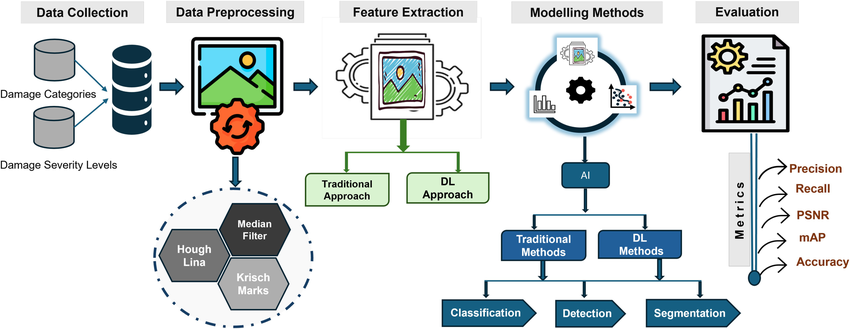
\includegraphics[scale=2]{Общая схема подходов CNN}
\caption{Обзор системы обнаружения повреждений транспортных средств \cite{src1}}
\end{figure}


Классификация - для определения типа повреждения/детали, обнаружение (детекция) - для определения местоположения, а сегментация - для выделения точных областей, обеспечения точности на уровне пикселей.


Проведённый глубокий поиск статей и источников показал, что возможности традиционных методов ограничены только простыми задачами классификации, такими как различения повреждённых и неповреждённых транспортных средств или определения базовых типов повреждений. По более сложным задачам научных статей обнаружено не было. Это объясняется тем, что определение границ поврежденных областей - трудная задача для традиционных методов по причине их зависимости от низкоуровневых объектов и ограниченного пространственного контекста. \cite{src1}. В одной из статей также ссылаются на источник, в котором проводилось исследование, показавшее, что в задаче обнаружения мелких повреждений в стальных канатах свёрточные нейронные сети значительно превосходят другие методы машинного обучения, такие как kNN, SVM, Random Forest и Logistic Regression. \cite{src6}


В подавляющем большинстве рассмотренных современных работ по распознаванию и классификации повреждений транспортных средств используются CNN-архитектуры для задач классификации, детекции и сегментации. Рассматриваемые методы нацелены на быстрый и информативный анализ изображений - именно экономия времени и ресурсов при сохранении требуемого уровня точности является основной целью исследований.

\section{Свёрточные нейронные сети в анализе изображений}\label{ch:1.1}

Глубокое обучение, в частности свёрточные нейронные сети (CNN), продемонстрировало впечатляющие результаты в широком спектре задач визуального распознавания, от обнаружения объектов до семантической сегментации \cite{src7} . 

Основная идея CNN заключается в последовательном выделении признаков с изображения, начиная с простых граней, текстур на первых уровнях и заканчивая сложными формами в более глубоких слоях. 

Типовая CNN состоит из последовательности сверточных слоёв, выделяющих локальные признаки изображения, и слоёв объединения (пуллинговых слоёв) для уменьшения размерности и устойчивости к смещению. После свёрток обычно идут полносвязные слои (или сверточные «головы») для предсказания классов или координат объектов. \cite{src14}

\begin{figure}[h]
\centering
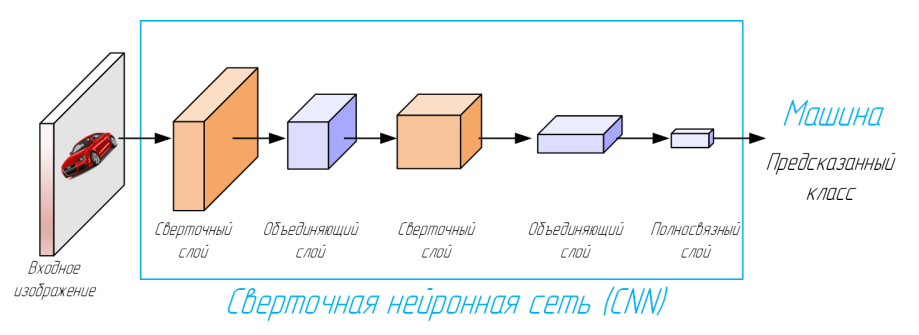
\includegraphics[scale=0.65]{Typical_CNN}
\caption{Концепция архитектуры CNN \cite{src14}}
\end{figure}


Такая архитектура позволяет выявлять сложные визуальные закономерности на изображении. Как отмечено в одном из источников, CNN особенно хороши в распознавании краёв, форм, текстур на изображениях, что делает их отличными помощниками в классификации изображений. \cite{src3}

Современные модели с CNN архитектурой можно разбить на две большие группы - одноэтапные и двухэтапные. 

Представителями двухэтапных методов является серия R-CNN. (Mask R-CNN, Faster R-CNN) Этот метод генерирует множество областей-кандидатов, которые могут содержать объекты, при первой обработке изображения. Затем для каждой области-кандидата производится повторная обработка через CNN. Это обеспечивает высокую точность предсказания, однако есть и главный недостаток: подход достаточно медленный и требует больших вычислительных ресурсов.
Поэтому был разработан алгоритм YOLO (You Only Look Once), впервые предложенный в 2016 году - он обрабатывает всё изображение "за один проход", что ускоряет обнаружение объектов. \cite{src2}

Серия YOLO получила широкую популярность благодаря балансу скорости и точности. Начиная с YOLOv5 и заканчивая YOLOv8, а в последнее время и YOLOv11, модели претерпели значительные архитектурные переработки, такие как улучшение базовых компонентов, подходов к агрегированию признаков и методов обучения, что в совокупности повысило эффективность обнаружения. Несмотря на улучшения и прочие достижения, в сфере обнаружения повреждений транспортных средств по-прежнему существуют проблемы. \cite{src7}

Рассмотрим более подробно существующие решения задачи оценки повреждений автомобилей.

\section{Разделение задачи на подзадачи: детали, повреждения и оценка стоимости}\label{ch:1.2}


Задача оценки повреждений достаточно масштабная. И нередко её разбивают на несколько взаимосвязанных этапов, таких как определение повреждений автомобиля и оценка стоимости. Так, в статье "Vehicle damage severity estimation for insurance operations using inthe-wild mobile images" описывается подход пайплайна подзадач: они обнаруживают автомобиль, затем проводят семантическую сегментацию всех его деталей и всех повреждённых участков, рассматривая и тот, и другой этап как задачу инстанс-сегментации с применением Mask R-CNN. После сегментации всех кузовных частей и всех повреждённых частей вычисляется относительная площадь повреждений по каждой детали, и затем передаётся в модель окончательной оценки стоимости ремонта. В работе шаг окончательной оценки стоимости и прочие шаги также выделяются как отдельные части пайплайна.  \cite{src9}

\begin{figure}[h]
\centering
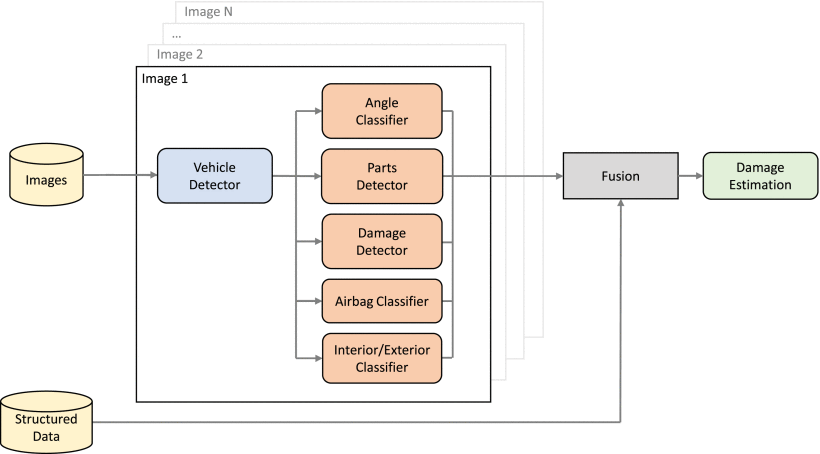
\includegraphics[scale=0.5]{Пайплайн}
\caption{Обзор пайплайна процесса оценки ущерба \cite{src9}}
\end{figure}

Такой подход имеет несколько преимуществ:

\begin{itemize}
   \item Это позволяет последовательно решать проблему, поэтапно выполняя действия по получению нужного результата от анализа изображения.
   \item Объекты разных типов (детали и повреждения) могут требовать разных подходов для необходимой точности обнаружения, а предварительное разбитие на подзадачи сегментации позволяет снять часть фона и точнее анализировать повреждения.
   \item Разделение на подзадачи позволяет выполнить его с помощью нескольких моделей (например, одна модель для сегментации деталей, а вторая - для повреждений). Это позволяет сначала обучить модель находить и классифицировать детали, а затем распознавать повреждения на уже вырезанных деталях
   \item Пайплайн из подзадач позволяет видеть промежуточные результаты и анализировать их. Ошибки и прочие проблемы на каждой из фаз общего процесса можно корректировать отдельно
\end{itemize}

Продолжая тему разделения ответственности решения на несколько этапов, рассмотрим подходы по детекции и классификации как деталей, так и повреждений.


\section{Подходы к распознаванию деталей автомобиля}\label{ch:1.3}


При анализе изображения на предмет обнаружения деталей автомобиля применяются как сегментационные, так и детекторные методы.
В ряде работ реализована инстанс-сегментация деталей, позволяющая выделять деталь отдельной маской. Существует множество алгоритмов сегментации, каждый из которых имеет свои преимущества и недостатки. 
В статье "Evaluation of deep learning algorithms for semantic segmentation of car parts" проведено сравнение пяти алгоритмов сегментации - Mask R-CNN, Hybrid Task Cascade (HTC), Composite Backbone Network (CBNet), Path Aggregation Network (PANet) и Global Context Network (GCNet)), в котором best-performing оказался HTC с ResNet-50 по метрике mAP. Авторы работы также оценивали устойчивость модели к зашумлённым данным (в частности, при плохих погодных условиях - туман, снегопад) и GCNet показала лучший результат по метрике mPC. \cite{src10}

Параллельно с сегментацией, детали часто определяют стандартной детекцией. Так, в работе "Optimized car parts detection with advanced feature fusion and attention modules" предложена улучшенная YOLO-архитектура для детекции мелких частей автомобиля. \cite{src11}

\subsection{Mask R-CNN}\label{ch:1.3.1}


Алгоритм сегментации объектов Mask R-CNN был разработан на основе Faster R-CNN. Его новизна заключается в том, что Faster R-CNN мог только определять местоположение объекта на изображении и распознавать его, а Mask R-CNN также может производить и сегментацию объектов.

Mask R-CNN состоит из двух основных частей:
\begin{itemize}
   \item Базовой модели (Backbone), которая извлекает признаки из изображения с помощью остаточной нейронной сети (ResNet), состоящей из 50–101 слоя свёрточной нейронной сети, в сочетании с сетью Feature Pyramid Network (FPN)
   \item "Головы" (Head), которая создаёт ограничивающую рамку (Bounding Box) вокруг интересующей области (ROI) и определяет тип объекта в этой рамке
\end{itemize}

Ещё одна особенность, отличающая Mask R-CNN от Faster R-CNN - создание маски для каждой области интереса (ROI).  \cite{src10}

\begin{figure}[h]
\centering
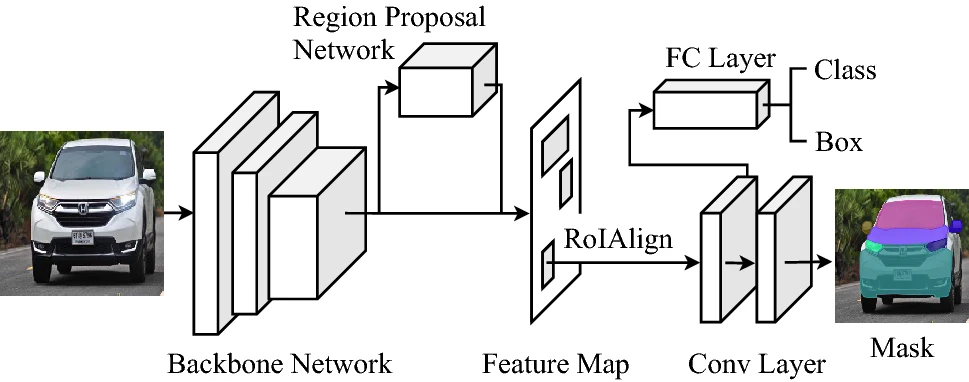
\includegraphics[scale=0.5]{Mask R-CNN}
\caption{Архитектура Mask R-CNN \cite{src10}}
\end{figure}


\subsection{Global Context Network (GCNet)}\label{ch:1.3.2}

Архитектура Global Context Network (GCNet) имеет структуру, схожую с Mask R-CNN, которая показана на рисунке 4. Однако особенностью GCNet является расширение Backbone блоком глобального контекста, схема которого отражена на рисунке 5.

\begin{figure}[h]
\centering
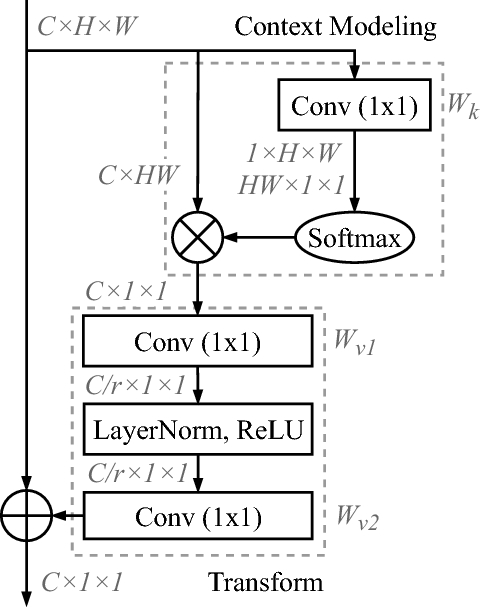
\includegraphics[scale=0.5]{GCNet}
\caption{Блок глобального контекста (Global Context). Карта признаков имеет размер C × H × W — количество каналов C, высота H и ширина W. × обозначает матричное умножение, а + — поэлементное сложение с трансляцией. r — коэффициент узкого места, а C/r — размерность скрытого представления узкого места \cite{src10}}
\end{figure}

Преимущество такого блока в том, что в его состав входит Non-Local Network (NLNet), помогающая решить проблему дальнодействующих зависимостей. \cite{src10}

\subsection{Hybrid Task Cascade (HTC)}\label{ch:1.3.3}

Алгоритм Hybrid Task Cascade (HTC) был создан с целью повышения эффективности инстанс-сегментации. 

Особенности:
\begin{itemize}
    \item В архитектуре блоки предсказания ограничивающих рамок (bounding box'ов), масок и извлечения ROI организованы в каскадную структуру, как показано на рисунке 6
    \item Процессы предсказания ограничивающих рамок и масок выполняются параллельно и последовательно на нескольких стадиях
    \item Многостадийная ветвь предсказания масок - маска, полученная на одном этапе, используется при генерации маски на следующем.
    \item Модель учитывает контекст при формировании каждой маски
\end{itemize}

\begin{figure}[h]
\centering
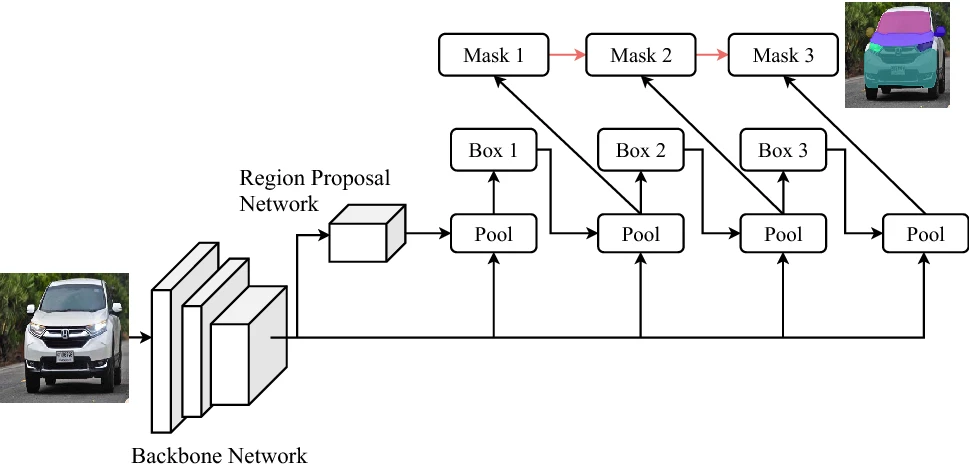
\includegraphics[scale=0.5]{HTC}
\caption{Архитектура HTC \cite{src10}}
\end{figure}

Совокупность этих улучшений существенно улучшает передачу информации между задачами и повышает итоговую точность. \cite{src10}

\subsection{Усовершенствованная архитектура на базе YOLO}\label{ch:1.3.4}

Важные особенности архитектуры:
\begin{itemize}
    \item Внедрён C2f (Cross Stage Partial style block) блок - помогает сохранять низкоуровневые признаки
    \item Внедрён модифицированный C2fCIB (C2f + Channel Interaction Block) блок - усиливает межканальные зависимости
    \item PSA (Pyramid Split Attention Module) - повышает выделение мелких/схожих деталей
\end{itemize}

\begin{figure}[h]
\centering
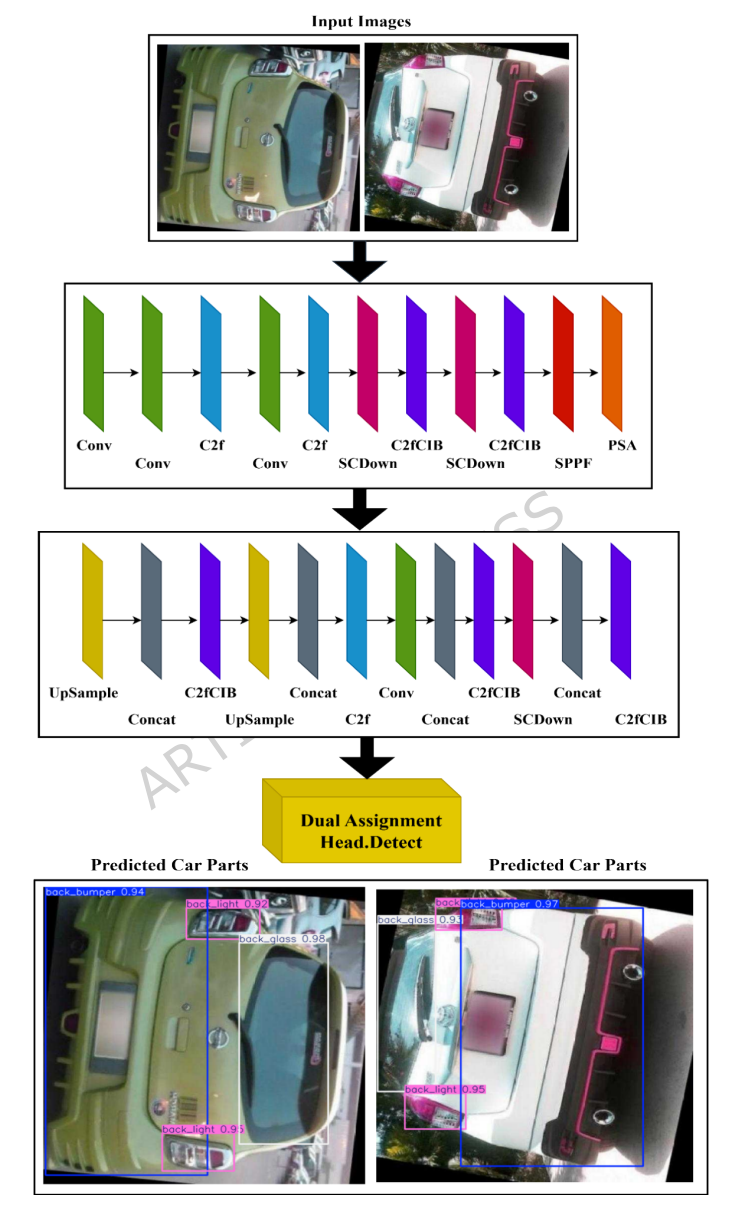
\includegraphics[scale=0.5]{improved_yolo}
\caption{Архитектура улучшенной YOLO \cite{src11}}
\end{figure}

Однако подход имеет и недостатки:
\begin{itemize}
    \item Очень мелкие части (<1\% изображения) всё так же остаются проблемой
    \item Модель стала заметно тяжелее по параметрам (3.2M параметров у YOLOv8 против 74.6M у предложенной модели) и требует куда больше вычислений. \cite{src11}
\end{itemize}

Результаты сравнения с другими подходами показали, что предложенные архитектурные улучшения дают существенный рост по метрикам Recall и mAP в задаче детекции деталей автомобиля. Авторский вариант YOLO превосходит некоторые классические двухэтапные R-CNN подходы, такие как Faster R-CNN и SSD, по метрикам Precision, Recall, mAP на рассматриваемом датасете car-parts.

\section{Подходы к распознаванию повреждений автомобиля}\label{ch:1.4}

Методы распознавания повреждений автомобиля, в отличие от задачи детекции автомобильных деталей, требуют более тщательного и точного анализа изображений. По мнению авторов статьи "Vehicle Damage Severity Estimation for Insurance Operations Using In-The-Wild Mobile Images", задача обнаружения повреждений скорее является задачей сегментации, а не задачей детекции, и многие современные методы отдают предпочтение именно сегментации. Сегментационные маски позволяют точнее описывать размытые очертания и мелкие дефекты, чем ограничивающие рамки (bounding box'ы). \cite{src9}

В статье "Automatic damaged vehicle estimator using enhanced deep learning algorithm" используют улучшенный Mask R-CNN с предварительно обученными моделями Inception-ResNetV2, VGG16, VGG19 для локализации и классификации повреждений. Комбинация Mask R-CNN с Inception-ResNetV2 показала лучшие результаты \cite{src4}

Популярны так же и решения с улучшенными YOLO-архитектурами специально для повреждений. 

Один из примером улучшенного YOLO - HL-YOLO. Это модифицированный YOLOv11, использующий гетерогенные свёртки и специальные механизмы внимания.

Особенности архитектуры:
\begin{itemize}
    \item Используются механизмы внимания для более точного выявления мелких и нерегулярных повреждений автомобиля, таких как царапины и вмятины.
    \item Применяется Large Separable Kernel Attention (LSKA), позволяющий учитывать пространственный контекст на больших расстояниях и повышать чувствительность к слабовыраженным, мелким дефектам.
    \item Дополнительным преимуществом HL-YOLO является использование модуля C3k2-HetConv, который включает гетерогенные свёртки и частичное разделение признаков. Это помогает одновременно и снизить вычислительные затраты, и повысить чувствительность к мелким повреждениям \cite{src7}
\end{itemize}

\begin{figure}[h]
\centering
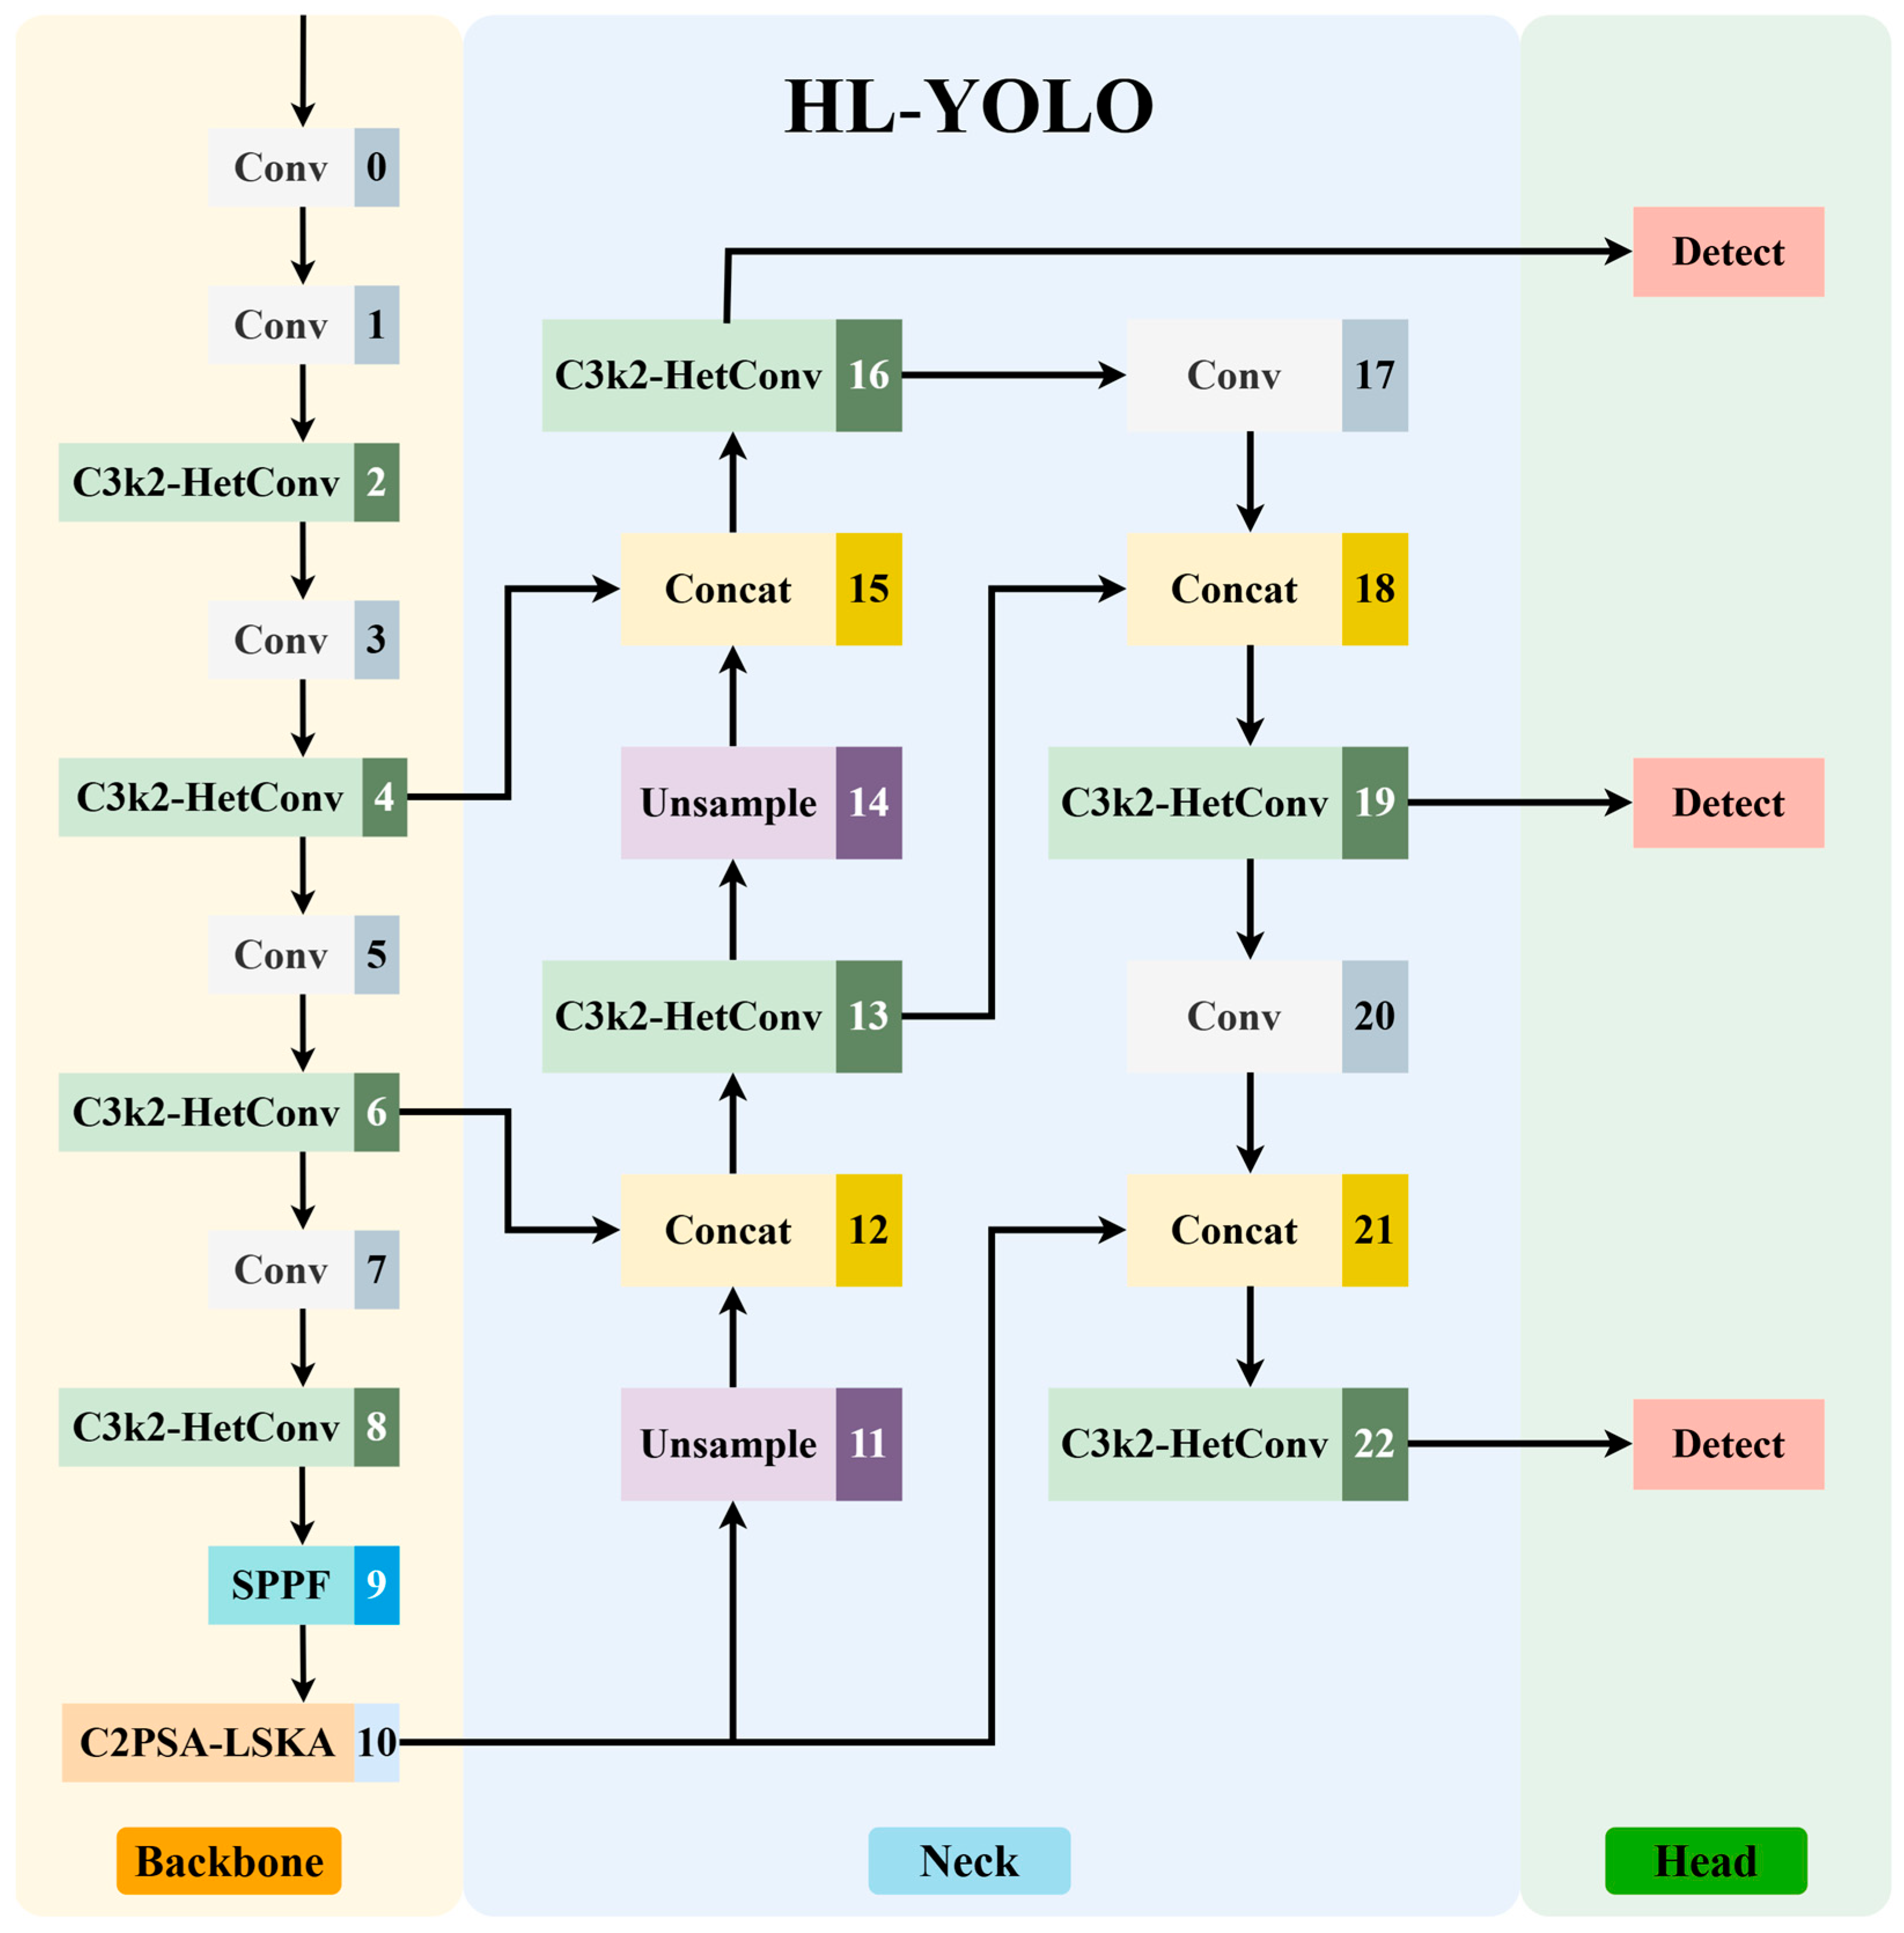
\includegraphics[scale=1]{hl_yolo}
\caption{Архитектура HL-YOLO \cite{src7}}
\end{figure}

Также в источнике "Small Dents, Big Impact: A Dataset and Deep Learning Approach for Vehicle Dent Detection" был проведён следующий эксперимент: собран датасет мелких вмятин и обучены YOLOv8-модели. Модель YOLOv8m-t42 достигла точности ~0.86 и полноты ~0.84 при обнаружении даже микроскопических вмятин. Полученные результаты указывают на то, что одностадийные детекторы тоже могут быть эффективны для этой узкой задачи нахождения повреждений. \cite{src12}

Проведённые сравнения моделей говорят о том, что выбор зависит от требований к точности и скорости. В одном из сравнений YOLO и Faster R-CNN  показано, что YOLO показывают результат по метрикам Recall и mAP немного хуже, чем Faster R-CNN, однако требуют меньше ресурсов (GFLOPs) и намного быстрее (FPS). \cite{src7}

\begin{figure}[h]
\centering
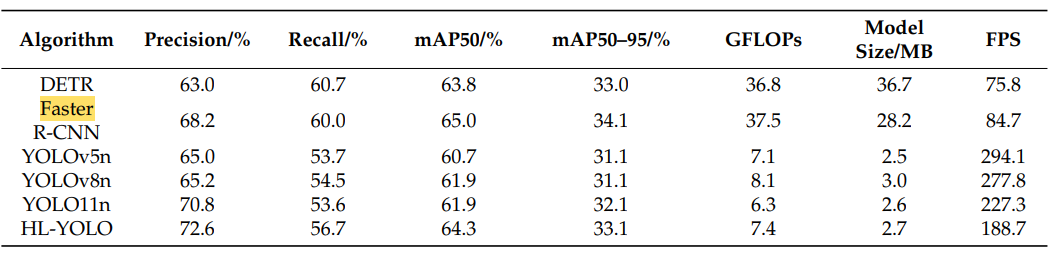
\includegraphics[scale=0.5]{yolo_vs_r_cnn}
\caption{Точность и эффективность различных моделей обнаружения \cite{src7}}
\end{figure}

Исследование показывает, что детекторы YOLO дают баланс скорости и точности, в то время как инстанс-сегментаторы типа Mask R-CNN могут обеспечивать более высокую точность (маски повреждений), но с использованием больших ресурсов.


\begin{table}[ht]
\caption{Архитектурные подходы к решению задачи оценки повреждений}
\label{table:simple_example}
\begin{tabularx}{\textwidth}{|>{\raggedright\arraybackslash}p{4.5cm}
                          |>{\raggedright\arraybackslash}X
                          |>{\raggedright\arraybackslash}X|}
\hline
\textbf{Описание архитектурного подхода} & \textbf{Минусы} & \textbf{Плюсы} \\
\hline
Общая модель и для деталей, и для повреждений
&
Сложнее обучать и интерпретировать результаты
&
Минимальное кол-во этапов обработки
\\
\hline
Пайплайн подзадач (детали и повреждения как отдельные шаги)
&
Увеличение числа этапов
&
Улучшенная управляемость, точность, возможность оптимизации каждого этапа
\\
\hline
\end{tabularx}
\end{table}



\begin{table}[ht]
\caption{Подходы(модели) для сегментации деталей автомобиля}
\label{table:simple_example}
\begin{tabularx}{\textwidth}{|>{\raggedright\arraybackslash}p{4.5cm}
                          |>{\raggedright\arraybackslash}X
                          |>{\raggedright\arraybackslash}X|}
\hline
\textbf{Описание подхода / модели} & \textbf{Минусы} & \textbf{Плюсы} \\
\hline
Mask R-CNN
&
Высокая сложность, скорость инференса ниже
&
Очень высокая точность масок, чёткое разделение деталей
\\
\hline
Hybrid Task Cascade (HTC)
&
Более сложная архитектура и обучение
&
Достаточно высокая точность - за счёт каскадного уточнения масок
\\
\hline
Global Context Network (GCNet)
&
Увеличение сложности модели
&
Устойчивость к нестандартным условиям съёмки, шумам
\\
\hline
YOLO-архитектуры
&
Могут выдавать недостаточно точные маски деталей
&
Высокая скорость обучения и инференса
\\
\hline
\end{tabularx}
\end{table}

\begin{table}[ht]
\caption{Подходы(модели) для сегментации повреждений автомобиля}
\label{table:simple_example}
\begin{tabularx}{\textwidth}{|>{\raggedright\arraybackslash}p{4.5cm}
                          |>{\raggedright\arraybackslash}X
                          |>{\raggedright\arraybackslash}X|}
\hline
\textbf{Описание модели} & \textbf{Минусы} & \textbf{Плюсы} \\
\hline
Mask R-CNN 
&
Требует точной разметки, много ресурсов, дольше инференс
&
Точно выделяет повреждения, лучше локализация
\\
\hline
YOLOv8
&
Может выдавать плохие результаты на сложных повреждениях
&
Баланс скорости и точности результатов
\\
\hline
Улучшенные YOLO-архитектуры
&
Недостаточно точные границы повреждений
&
Повышенная чувствительность к мелким дефектам
\\
\hline
\end{tabularx}
\end{table}

\begin{table}[ht]
\caption{Сравнение двухэтапных и одноэтапных подходов}
\label{table:simple_example}
\begin{tabularx}{\textwidth}{|>{\raggedright\arraybackslash}p{4.5cm}
                          |>{\raggedright\arraybackslash}X
                          |>{\raggedright\arraybackslash}X|}
\hline
\textbf{Подход} & \textbf{Минусы} & \textbf{Плюсы} \\
\hline
Двухэтапные (Mask R-CNN, HTC и др.)
&
Медленные, требовательны к ресурсам и точной разметке
&
Максимальная точность сегментации
\\
\hline
Одноэтапные (YOLO и модификации)
&
Менее точные маски
&
Высокая скорость и более простое обучение
\\
\hline
\end{tabularx}
\end{table}

\chapter{Структурный системный анализ исследуемого объекта}\label{ch:2}

Объектом исследования в данной работе является процесс оценки стоимости ремонта автомобилей в автосервисе. Процесс достаточно обширен и включает в себя множество действий, начиная от обращения клиента и заканчивая принятием решения о начале ремонтных работ (либо отказом). В него вовлечены три основные роли:

\begin{itemize}
    \item Клиент
    \item Сотрудник автосервиса (мастер)
    \item Начальник автосервиса
\end{itemize}

Для погружения в контекст процесса и понимания его деталей, была составлена BPMN-диаграмма, подробно отражающая состояние "as is" в автосервисе. (Рисунок 10)


Проанализировав диаграмму, можно выявить основные проблемные места процесса:
\begin{itemize}
    \item Не все клиенты обращаются в автосервис лично. Многие делают это в режиме онлайн, и этап сбора информации сопряжён с дополнительными трудностями. Иногда может быть недоступен сотрудник автосервиса, к которому обращаются, и клиенту приходится ожидать, пока мастер дойдёт до устройства, обработает обращение и даст обратную связь.
    \item Несогласованный формат отправки изображений мастеру приводит к тому, что иногда информации с изображений недостаточно (например, не понятно, что за деталь), и приходится запрашивать уточнение данных или новое фото. Это приводит к затратам времени на переписку (дополнительные циклы пересъёмки/разъяснений, ожиданий ответа с обеих сторон).
    \item Иногда неопытность сотрудника и отсутствие чёткого понимания расценки работ приводит либо к необходимости согласования с начальником автосервиса (дополнительное время на согласование), либо к тому, что одна и та же поломка может оцениваться по-разному разными мастерами. 
\end{itemize}

\begin{figure}[H]
\centering
\begin{minipage}{0.90\textwidth}
    \centering
    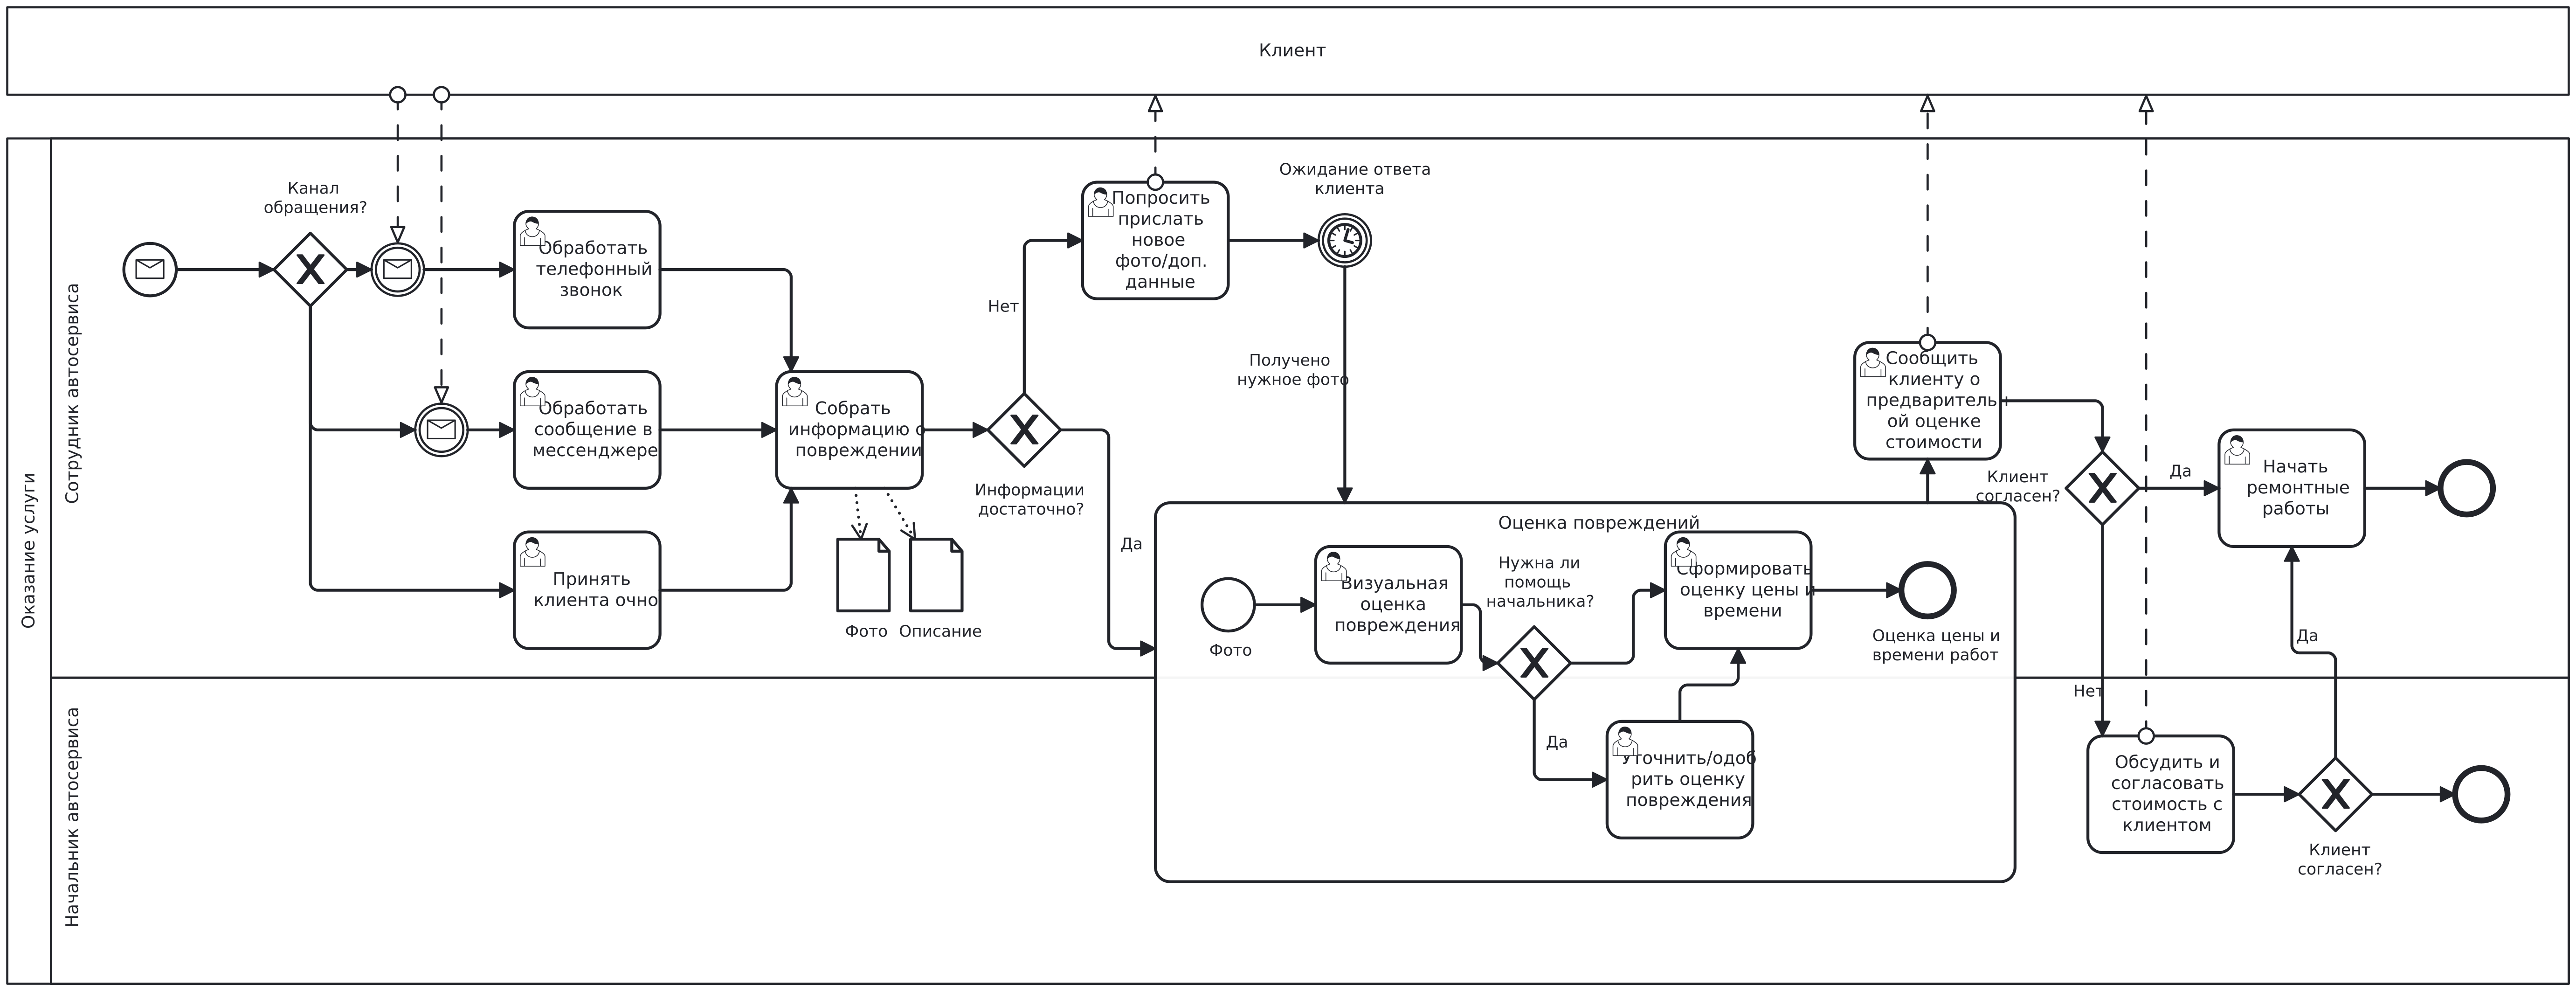
\includegraphics[scale=0.55, angle=90]{BPMN}
\end{minipage}\hspace{-4em}%
\begin{minipage}{0.06\textwidth}
    \centering
    \rotatebox{90}{%
        \parbox{10cm}{\caption{BPMN-диаграмма процесса}}%
    }
\end{minipage}
\end{figure}

По экспертной информации, предоставленной начальником автосервиса, более половины случаев обрабатываются в режиме онлайн, а время обработки одного онлайн-обращения занимает в среднем 30 минут. Это указывает на высокую загруженность мастеров в дни обработки обращений сразу от множества клиентов. Около 20\% обращений обсуждаются с начальником, а с клиентом контакты осуществляются в среднем 2-3 раза, что также говорит о весомых тратах времени на согласование.

Таким образом, в текущем бизнес-процессе имеется несколько существенных недостатков:
\begin{itemize}
    \item Длительные согласования и ожидания ответа
    \item Отвлечение мастеров от работы на приём обращений
    \item Ошибки при оценке стоимости у новых сотрудников
\end{itemize}

По имеющейся статистике, вероятность существенного изменения (более, чем на 5-10\%) предварительной оценки стоимости ремонта - всего около 5\%. Это указывает на устойчивость и воспроизводимость результатов предварительной оценки.
% \chapter{Анализ технического, программного и информационного обеспечений}\label{ch:3}

\section{Анализ технического обеспечения}\label{sec:3.1}

Техническое обеспечение процесса предварительной оценки повреждений автомобилей по сути отсутствует. 

\begin{itemize}
    \item Клиентские устройства. Фотографии повреждений поступают преимущественно с мобильных устройств клиентов (смартфонов) через мессенджеры. Сотрудники автосервиса также используют мобильные устройства и/или персональные компьютеры для просмотра изображений и подготовки ответов.
    \item Сетевое подключение. Обмен изображениями осуществляется через Интернет и инфраструктуру мессенджеров. Специально выделенных сетей или VPN нет.
\end{itemize}

На текущем этапе нет каких-либо хранилищ или баз данных для систематического хранения фото и прочих метаданных: все изображения и информация о клиенте остаются в чатах мессенджеров и/или локально на устройствах сотрудников.
Резервное копирование не проводится.

Отсутствие какой-либо стандартизированной инфраструктуры приводит к невозможности систематизировать данные, к трудностям в аналитике и масштабировании, низкой отказоустойчивости процесса.

\section{Анализ программного обеспечения}\label{sec:3.2}

В текущем процессе отсутствует специализированное программное обеспечение. Клиенты используют только набор приложений без специализированного ПО для учёта, обработки и систематизации заявок.
Мессенджеры - основной канал приёма и обмена фотографиями. Клиенты присылают фото в личные чаты, сотрудники автосервиса дают ответы и проводят согласование.

\section{Анализ информационного обеспечения}\label{sec:3.3}

Основной источник информации — фотографии, присылаемые клиентами в мессенджеры. Текстовые сообщения с описанием повреждений отправляются клиентами в те же чаты.
Отсутствует какая-либо стандартизация формата присылаемых данных - изображения/описание повреждения могут прислать в любом виде, что и зачастую приводит к проблеме недостатка информации и трате времени на дополнительное обсуждение деталей.
Информация о состоянии обращения также нигде не хранится и сообщается клиенту лишь при наступлении определённого события, например, при завершении ремонта. 

\chapter{Постановка задачи}\label{ch:4}

Структурный системный анализ объекта исследования показал, что значительная доля заявок клиентов поступает в виде фотографий, а процесс обработки обращений имеет множество недостатков, таких как длительные ожидания и согласования, просчёты новых сотрудников. Устойчивость и воспроизводимость результатов предварительной оценки подтверждает возможность и необходимость внедрения автоматизированного сервиса оценки повреждений автомобилей по фотографии.

Цель работы - повышение эффективности процесса оценки стоимости ремонта поврежденных автомобилей. Был сформулирован список задач, которые необходимо выполнить для достижения цели:

\begin{enumerate}[label=\arabic*.]
    \item Сформировать датасет для обучения модели путём сбора и фильтрации изображений повреждённых автомобилей и их дальнейшей разметки. 
    \item Разработать модули для обработки и аугментации изображений, устранения недостатков съёмки
    \item Обучить ML-модель обнаружения и классификации деталей и повреждений на основе размеченных данных
    \item Реализовать бизнес-логику оценки стоимости и длительности ремонта
    \item Спроектировать и реализовать микросервисную архитектуру приложения, описать и произвести процесс интеграции с ботом в мессенджере
    \item Описать и разработать архитектуру базы данных
    \item Интеграция CI/CD и процесса поставки программного обеспечения
    \item Провести тестирование работоспособности системы
\end{enumerate}

Предполагаемым результатом работы является реализованный сервис с внедрённой в него ML-моделью распознавания и классификации повреждений автомобиля. 

Эффективность решения можно будет оценить двум основным факторам:
\begin{enumerate}[label=\arabic*.]
    \item Производительность системы
    \begin{itemize}
        \item Время обработки одного изображения
        \item Пропускная способность сервисов (RPS) 
    \end{itemize}
    \item Минимизация человеческого участия - на сколько уменьшится время обработки обращений клиентов
\end{enumerate}
\chapter{Архитектурно-техническое решение задачи}\label{ch:5}

При проведении структурного системного анализа была создана модель "'as is"', которая показала, что значительная часть работы выполняется вручную. Мастера автосервиса тратят большое количество времени на общение с клиентом в мессенджере, анализ фотографий и получение информации, формирование предварительной оценки. Такой подход требует лишних временных затрат и увеличивает нагрузку на сотрудников. 

Чтобы решить описанную выше проблему, рассмотрим внедрение интеллектуальной системы в текущий процесс на BPMN-диаграмме "to be". (Рисунок 11). В диаграмме значительная часть операций текущего процесса передаётся новой автоматизированной системе.
Функционал, предоставляемый системой для пользователя, должен включать:

\begin{enumerate}[label=\arabic*.]
    \item Начало взаимодействия с системой через мессенджер. Пользователь имеет возможность написать боту и выбрать режим работы системы
    \item Выбор способа указания повреждений автомобиля. Система должна обеспечивать возможность выбрать один из двух способов указания повреждений:
    \begin{itemize}
        \item Указать повреждения и их типы через интерфейс бота
        \item Отправить фотографию повреждённого автомобиля, которую автоматически проанализирует система
    \end{itemize}
    \item Если пользователь выбрал автоматический режим:
    \begin{itemize}
        \item Система должна автоматически выполнить обработку и анализ фотографии с использованием методов машинного обучения: определить видимые детали автомобиля, имеющиеся на них повреждения и сформировать аннотированное изображение с выделенными масками деталей и повреждений.
        Должны обнаруживаться следующие детали:
        \begin{itemize}
            \item Дверь
		    \item Переднее крыло
		    \item Заднее крыло
		    \item Бампер
		    \item Багажник
		    \item Капот
		    \item Фара
		    \item Переднее стекло
		    \item Заднее стекло
		    \item Боковое стекло
		    \item Шины и в целом колёса
        \end{itemize}
        Должны обнаруживаться следующие повреждения:
        \begin{itemize}
            \item Царапина
		    \item Вмятина
		    \item Отвалившийся кусок краски
		    \item Ржавчина
		    \item Трещина
		    \item Разрывы/разрезы/дырки
	        \item Разбитые стекло или фары
		    \item Спущенные шины и любые проблемы с колёсами
        \end{itemize}
        \item Пользователь должен иметь возможность посмотреть результат автоматического анализа перед переходом к этапу расчёта стоимости ремонта. 
        \item Пользователь должен иметь возможность отредактировать результат анализа через интерфейс бота, если он не согласен с результатом, выданным моделью:
        \begin{itemize}
            \item Изменить тип повреждения
            \item Изменить принадлежность повреждения к детали автомобиля
            \item Удалить ошибочно найденное повреждение
            \item Добавить новое необнаруженное повреждение
        \end{itemize}
    \end{itemize}
    \item После проверки пользователем всех параметров повреждений система должна предоставить ему возможность подтвердить итоговый список повреждений автомобиля, чтобы перейти к расчёту.
    \item После подтверждения от пользователя система должна приступить к автоматическому расчёту ориентировочных стоимости и длительности работ в автосервисе согласно заданным параметрам, сопоставив их с правилами расчёта автосервиса (Таблицы 5 и 6)
    \item Пользователь должен получить сообщение с результатами расчёта, включающими стоимость и длительность ремонтных работ. 
\end{enumerate}


\begin{figure}[H]
\centering
\begin{minipage}{0.90\textwidth}
    \centering
    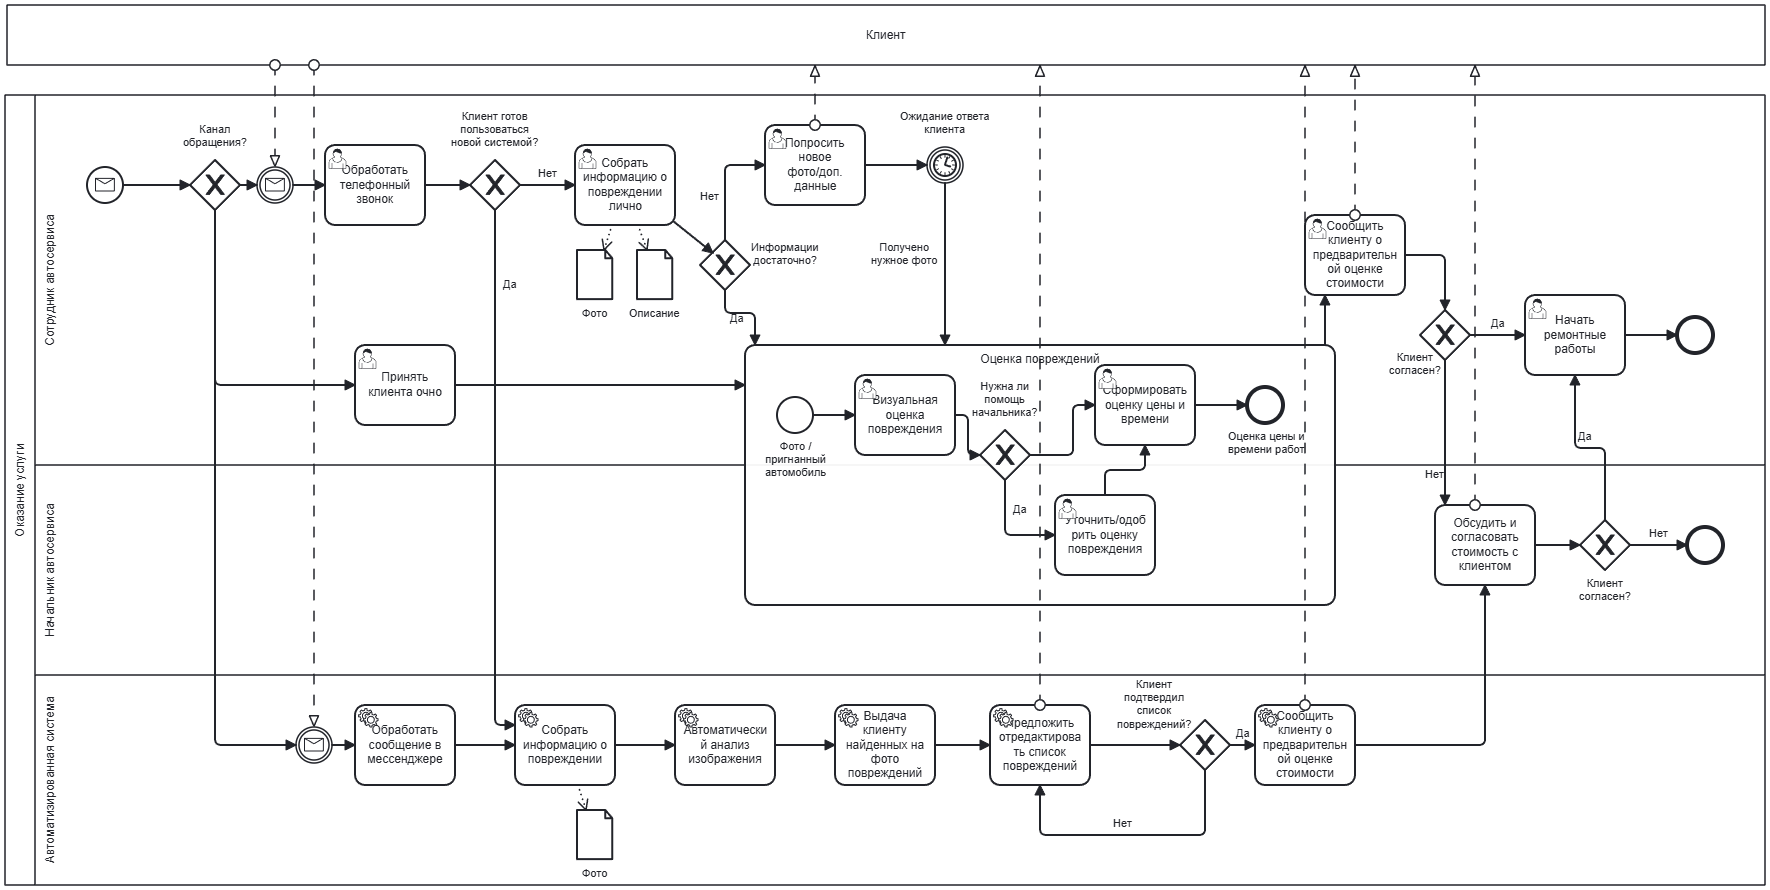
\includegraphics[scale=0.4, angle=90]{BPMN_to_be}
\end{minipage}\hspace{-2em}%
\begin{minipage}{0.06\textwidth}
    \centering
    \rotatebox{90}{%
        \parbox{10cm}{\caption{BPMN-диаграмма TO BE}}%
    }
\end{minipage}
\end{figure}

% \begin{table}[htbp]
% \centering
% \caption{Стоимость ремонта (тыс. руб.)}

% \begin{adjustbox}{max width=\textwidth}
% \begin{tabular}{lcccc}
% \hline
% Деталь & Царапина (полировка) & Царапина (покраска) & Вмятина (рихтовка + покраска) & Замена детали \\
% \hline

% Переднее крыло & 1 & 10--18 & 23--30 & 20 \\
% Заднее крыло & 1 & 10--18 & 23--30 & 75--100 \\
% Дверь & 1 & 10--18 & 23--30 & 20 \\
% Крышка багажника & 1 & 10--18 & 23--30 & 20 \\

% Порог & 1 & 10--18 & 23--30 & 50--55 \\
% Крыша & 1 & 10--18 & 23--30 & 75--100 \\

% Капот & 1 & 10--18 & 30--35 & 28--30 \\

% Бампер & 1 & 10--18 & 3--5 & 18 \\

% Лобовое стекло & --- & --- & --- & 5+ \\
% Боковое стекло & --- & --- & --- & 3 \\
% Фара & --- & --- & --- & 3 \\

% \hline
% \end{tabular}
% \end{adjustbox}

% \end{table}


% \begin{table}[htbp]
% \centering
% \caption{Длительность ремонта}

% \begin{adjustbox}{max width=\textwidth}
% \begin{tabular}{lcccc}
% \hline
% Деталь & Царапина (полировка) & Царапина (покраска) & Вмятина (рихтовка + покраска) & Замена детали \\
% \hline

% Переднее крыло & 1 час & 1 день & 2--3 дня & 1 день \\
% Заднее крыло & 1 час & 1 день & 2--3 дня & 5 дней \\
% Дверь & 1 час & 1 день & 2--3 дня & 1.5--2 дня \\
% Крышка багажника & 1 час & 1 день & 2--3 дня & 1.5--2 дня \\

% Порог & 1 час & 1 день & 2--3 дня & 1 день \\
% Крыша & 1 час & 1 день & 2--3 дня & 5 дней \\

% Капот & 1 час & 1 день & 2 дня & 2 дня \\

% Бампер & 1 час & 1 день & 1--2 дня & 1.5 дня \\

% Лобовое стекло & --- & --- & --- & 3 часа (оставить на день) \\
% Боковое стекло & --- & --- & --- & 1 день \\
% Фара & --- & --- & --- & 0.5 дня \\

% \hline
% \end{tabular}
% \end{adjustbox}

% \end{table}



\begin{table}[htbp]
\centering
\caption{Стоимость ремонта, тыс. руб.}
\begin{adjustbox}{max width=\textwidth}
\begin{tabular}{|l|c|c|c|c|}
\hline
Деталь & \begin{tabular}[c]{@{}c@{}}Царапина\\ (полировка)\end{tabular} & 
\begin{tabular}[c]{@{}c@{}}Царапина\\ (покраска)\end{tabular} & 
\begin{tabular}[c]{@{}c@{}}Вмятина\\ (рихтовка + покраска)\end{tabular} & 
Замена детали \\
\hline

Переднее крыло & 1 & 10–18 & 23–30 & 20 \\
Заднее крыло & 1 & 10–18 & 23–30 & 75–100 \\
Дверь & 1 & 10–18 & 23–30 & 20 \\
Крышка багажника & 1 & 10–18 & 23–30 & 20 \\

% Порог & 1 & 10–18 & 23–30 & 50–55 \\
Крыша & 1 & 10–18 & 23–30 & 75–100 \\

Капот & 1 & 10–18 & 30–35 & 28–30 \\

Бампер & 1 & 10–18 & 3–5 & 18 \\

Лобовое стекло & — & — & — & 5-10 \\
Боковое стекло & — & — & — & 3 \\
Фара & — & — & — & 3 \\

\hline
\end{tabular}
\end{adjustbox}
\end{table}

\begin{table}[htbp]
\centering
\caption{Длительность ремонта}
\begin{adjustbox}{max width=\textwidth}
\begin{tabular}{|l|c|c|c|c|}
\hline
Деталь & \begin{tabular}[c]{@{}c@{}}Царапина\\ (полировка)\end{tabular} & 
\begin{tabular}[c]{@{}c@{}}Царапина\\ (покраска)\end{tabular} & 
\begin{tabular}[c]{@{}c@{}}Вмятина\\ (рихтовка + покраска)\end{tabular} & 
Замена детали \\
\hline

Переднее крыло & 1 час & 1 день & 2–3 дня & 1 день \\
Заднее крыло & 1 час & 1 день & 2–3 дня & 5 дней \\
Дверь & 1 час & 1 день & 2–3 дня & 1.5–2 дня \\
Крышка багажника & 1 час & 1 день & 2–3 дня & 1.5–2 дня \\

% Порог & 1 час & 1 день & 2–3 дня & 1 день \\
Крыша & 1 час & 1 день & 2–3 дня & 5 дней \\

Капот & 1 час & 1 день & 2 дня & 2 дня \\

Бампер & 1 час & 1 день & 1–2 дня & 1.5 дня \\

Лобовое стекло & — & — & — & 1 день \\
Боковое стекло & — & — & — & 1 день \\
Фара & — & — & — & 0.5 дня \\

\hline
\end{tabular}
\end{adjustbox}
\end{table}




После выполнения всех шагов выше клиент сможет проще принять решение о пользовании услугами автосервиса, и сделать лишь финальный звонок сотруднику автосервиса (о времени визита / согласовании цены).

Предлагаемое решение, встроенное в текущий процесс, имеет несколько преимуществ:

\begin{enumerate}[label=\arabic*.]
    \item При поступлении обращения через канал мессенджера можно полностью передать управление системе - клиенту достаточно будет отправить фотографию или самостоятельно указать все имеющиеся повреждения.
    \item Сотруднику автосервиса не требуется проводить долгое общение в мессенджере для формирования ответа по стоимости - в системе клиент это может сделать самостоятельно, и, благодаря удобному интерфейсу, быстро задать параметры и получить ответ.
    \item Помимо полной автоматизации процесса при поступлении обращений через мессенджеры, можно предлагать клиентам пользоваться системой и при поступлении телефонных звонков - это также будет кратно экономить время.
\end{enumerate}

Для реализации функционала необходимо разработать приложение, которое будет обеспечивать описанные сценарии. Архитектура и математическая модель системы будут рассмотрены в следующем разделе.


\chapter{Математическая модель решения задачи}\label{ch:6}

\section{Архитектура решения в нотации C4}

Перед началом разработки приложения рассмотрим архитектуру будущего решения в виде нотации C4 - она представлена на рисунках 12-15. 

На рисунке 12 изображен уровень системного контекста - здесь отражено взаимодействие клиента с системой. Посредником в этом процессе является мессенджер, через интерфейс которого пользователю будет удобно взаимодействовать с системой.

\begin{figure}[h]
\centering
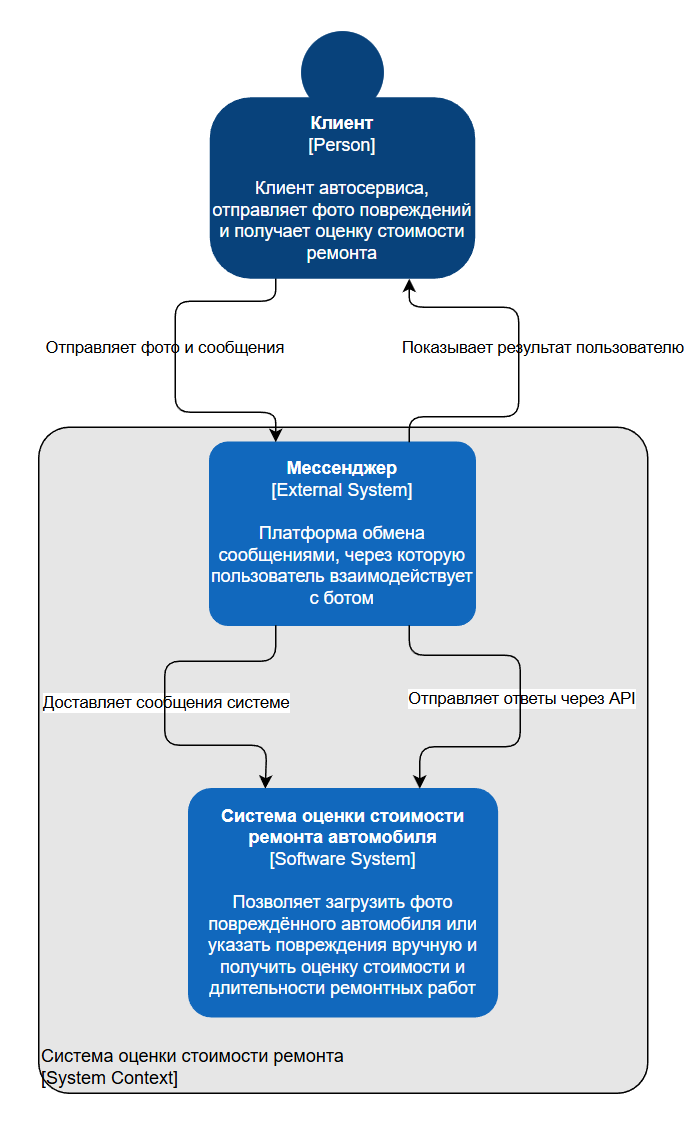
\includegraphics[scale=0.5]{c4_system_context}
\caption{Уровень системного контекста в нотации C4}
\end{figure}

\begin{figure}[h]
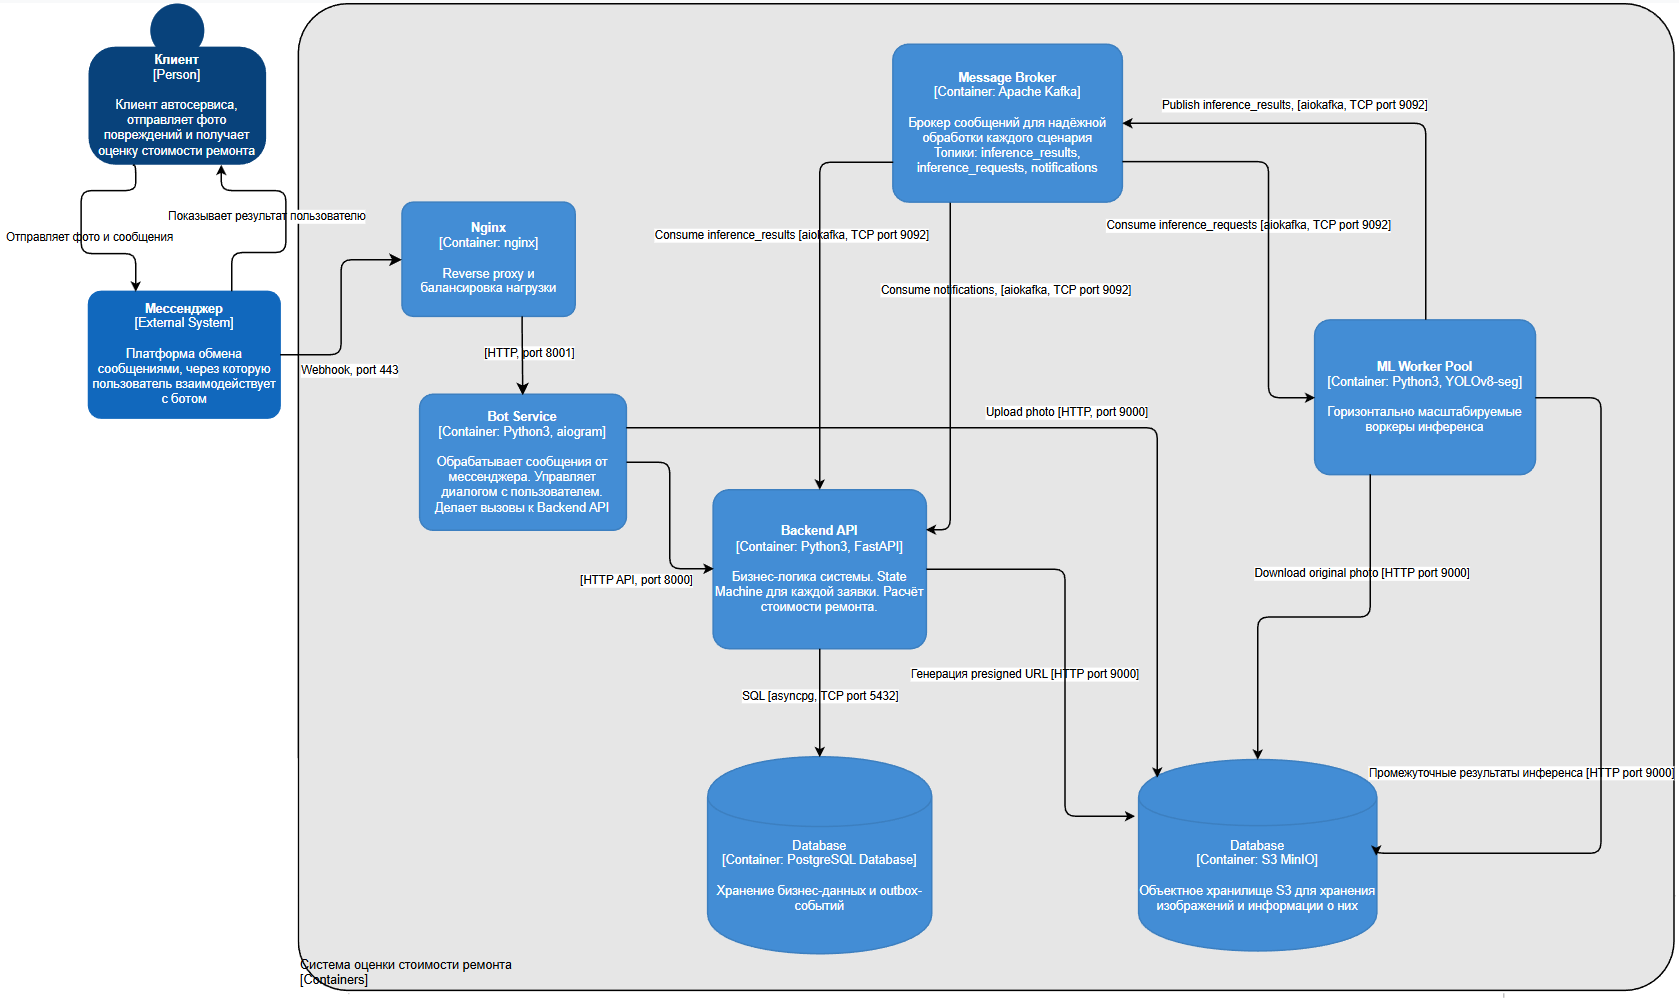
\includegraphics[scale=0.37]{c4_containers}
\caption{Уровень контейнеров в нотации C4}
\end{figure}

На рисунке 13 представлен контейнерный уровень. Здесь раскрываются подробности внутренней архитектуры системы оценки стоимости ремонтных работ. На схеме показана информация о следующих элементах системы и их взаимодействии:

\begin{itemize}
    \item Bot Service - принимает сообщения от пользователя мессенджера, преобразует их, отправляет системе и возвращает ответы пользователю
    \item Backend API - главный серверный компонент, в котором сосредоточена основная бизнес-логика:
        \begin{itemize}
            \item Управление сценарием обработки обращений и расчёт стоимости работ
            \item Взаимодействие с базами данных
            \item Взаимодействие с брокером сообщений
        \end{itemize}
    \item Nginx - обратный прокси-сервер, принимающий входящие запросы. Балансировщик нагрузки
    \item Message Broker (Kafka) - брокер сообщений, обеспечивающий отказоустойчивое взаимодействие между бэкендом и ML
    \item ML Worker Pool - пул обработчиков для анализа изображений
    \item PostgreSQL - реляционная база данных для хранения служебных данных - информации о сценариях, статусах, результатах и др.
    \item MinIO S3 - объектное хранилище для хранения исходных и аннотированных изображений
\end{itemize}

\begin{figure}[h]
\centering
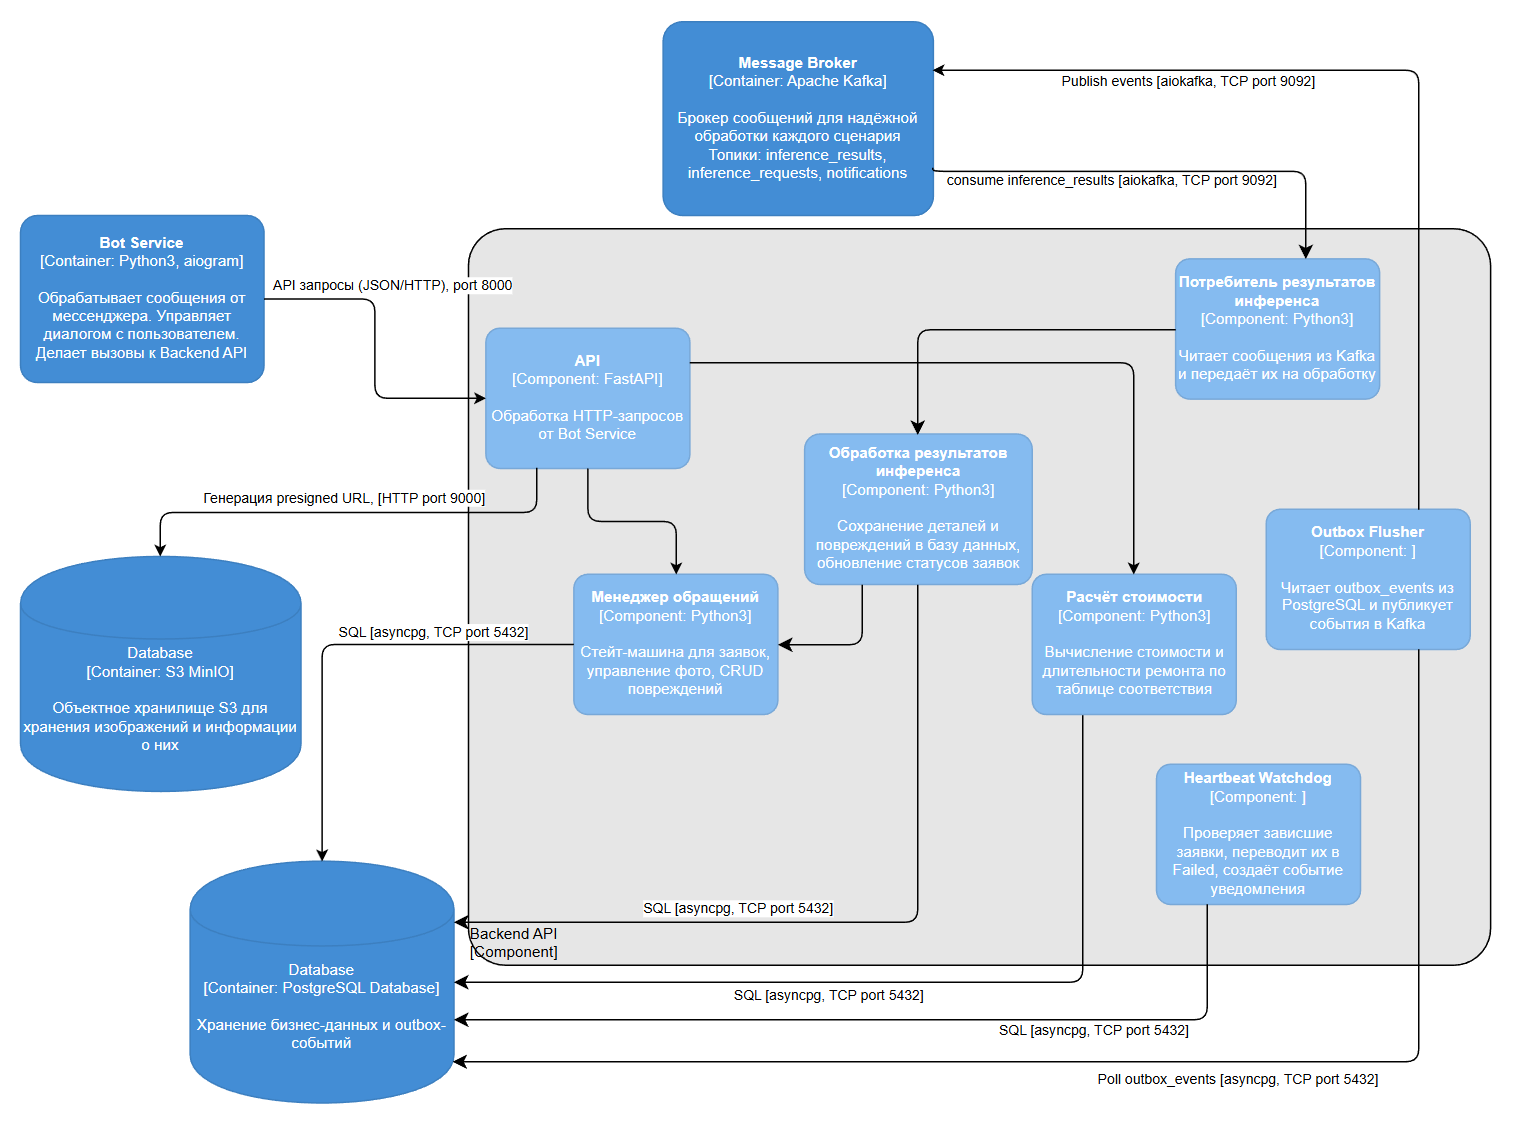
\includegraphics[scale=0.4]{c4_backend_api}
\caption{Компонентный уровень C4 - контейнер Backend API}
\end{figure}

Рассмотрим более подробно изнутри архитектуру самых важных частей системы - контейнеров Backend API и ML Worker'а.

Переходя к компонентному уровню нотации C4, начнём с контейнера бэкенда, в котором сосредоточена большая часть бизнес-логики (рисунок 14). От Bot Service'а к нему поступают запросы, которые обрабатываются компонентом API, использующем библиотеку FastAPI. Внутри реализуется стейт-машина и управление полным сценарием от отправки запроса в сервис инференса до получения ответа, взаимодействия с базами данных. Внутри контейнера имеются компоненты, позволяющие отказоустойчиво обработать каждый сценарий и отправить ответ пользователю, среди них:
\begin{itemize}
    \item Outbox Flusher - компонент для отказоустойчивой отправки накопленных событий из таблицы outbox в брокер сообщений
    \item Heartbeat Watchdog - компонент мониторинга зависших сценариев
\end{itemize}

\begin{figure}[h]
\centering
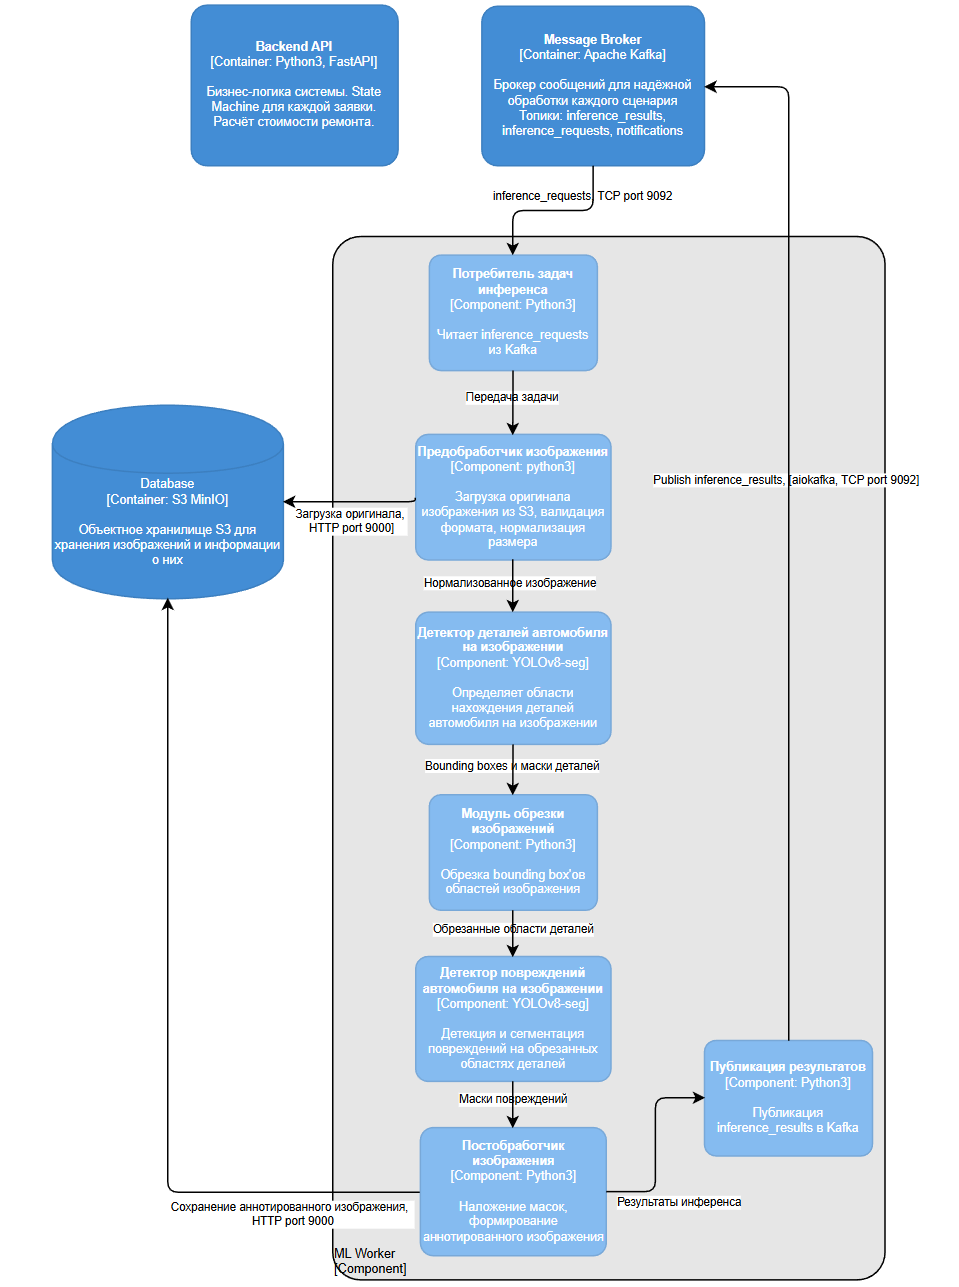
\includegraphics[scale=0.5]{c4_ml_worker}
\caption{Компонентный уровень C4 - контейнер ML Worker}
\end{figure}

Бэкенд взаимодействует с ML Worker'ами через брокер сообщений. Конечный вердикт по стоимости и длительности работ выполняется при помощи компонента расчёта стоимости.

Детальный обзор ML контейнера представлен на рисунке 15. Он получает сообщение от брокера сообщений о появившихся сценариях и производит цикл действий по обработке фотографии вплоть до формирования финального аннотированного изображения, которое сохраняет в S3. ML Worker состоит из следующих компонентов:
\begin{itemize}
    \item Предобработчик изображений - отвечает за подготовку изображения к анализу
    \item Детектор деталей автомобиля на изображении - определяет области расположения деталей
    \item Модуль обрезки изображений - отвечает за обрезку отдельных фрагментов изображения (деталей) по найденным областям
    \item Детектор повреждений автомобиля на изображении - определяет области расположения повреждений на обрезанных областях деталей
    \item Постобработчик изображения - формирует итоговое размеченное изображение 
\end{itemize}

\section{Схема базы данных}

\begin{figure}[h]
\centering
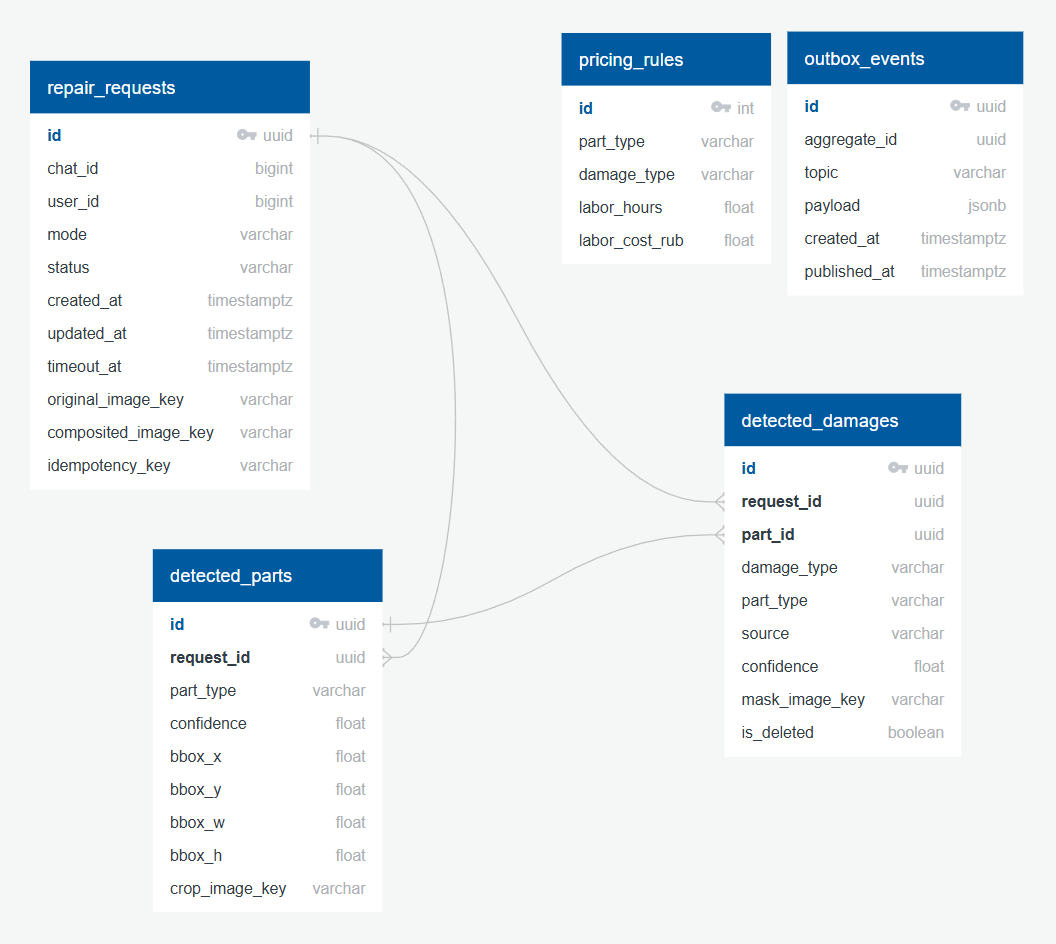
\includegraphics[scale=0.6]{db_schema}
\caption{Схема базы данных PostgreSQL}
\end{figure}

В системе имеется два хранилища данных - S3 MinIO для изображений и PostgreSQL для хранения данных о каждом сценарии и изображении. Рассмотрим схему базы данных PostgreSQL подробнее. Она создаётся скриптом инициализации при первом запуске контейнера и содержит несколько таблиц:

\begin{itemize}
    \item repair\_requests - хранение информации о заявке на оценку стоимости: информация о чате с пользователем, статусе, режиме обработки, изображении.
    \item detected\_parts - информация о результате сегментации деталей - тип детали, уверенность, ограничивающий прямоугольник
    \item detected\_damages - информация о найденных повреждениях - тип повреждения, уверенность, маска на изображении
    \item pricing\_rules - таблица для этапа расчёта стоимости и длительности работ на основе параметров <деталь - повреждение>
    \item outbox\_events - доменные события для Kafka
\end{itemize}

Визуализированная схема базы данных PostgreSQL с показанными связями и типами данных представлена на рисунке 16.



\section{Архитектура и математическая модель ML-составляющей}

Рассмотрим более подробно архитектуру контейнера ML Worker. Процесс внутри представлен в виде пайплайна подзадач - общий процесс детекции и сегментации повреждений разделён на несколько этапов, главными из которых являются компоненты, требующие обучения моделей детекции и сегментации деталей и повреждений (Причины выбора такого подхода описаны в главе 1).

Для решения задачи анализа изображения целесообразно выбрать модель семейства YOLO. Полноценное сравнение и анализ архитектур моделей производились в главе 1, и текущий выбор обусловлен тем, что YOLOv8 представляет собой компромисс между скоростью обучения и внедрения, скоростью инференса, вычислительной эффективностью и качеством предсказания.

В обобщённом виде архитектуру YOLOv8-seg можно представить как совокупность трёх частей:
\begin{itemize}
    \item backbone - извлечение признаков из входного изображения
    \item neck - объединение признаков разных масштабов
    \item segment head - предсказание классов, координат объектов и коэффициентов масок
\end{itemize}

Для обучения модели используются изображения повреждённых автомобилей. Подготовка данных и обучение поддерживают механизмы аугментации, включая Mosaic - преобразование, при котором несколько изображений объединяются в одно для улучшения обобщающей способности модели.

\subsection{Модель детекции и сегментации деталей автомобиля}

На вход системы поступает изображение автомобиля:
\[
X \in \mathbb{R}^{H \times W \times 3},
\]
где $H$ --- высота изображения, $W$ --- ширина изображения, а третье измерение соответствует цветовым каналам.

Перед передачей изображения в модель выполняется предобработка: изображение приводится к размеру входа модели 640 х 640 пикселей, а значения пикселей масштабируются к диапазону [0,1] путём деления на 255. Согласно документации Ultralytics \cite{src22}, такая схема соответствует стандартному способу подготовки данных для YOLO-моделей.

Первый этап пайплайна - изображение автомобиля обрабатывается моделью детекции и сегментации деталей. Обученная модель сегментации отображает входное изображение в множество предсказаний, каждое из которых содержит bounding box, маску, класс и confidence.

Результатом работы модели деталей является множество:
\[
S_{\text{parts}} = \left\{(b_i, m_i, p_i, s_i)\right\}_{i=1}^{N},
\]
где:
\begin{itemize}
    \item $b_i$ - bounding box (ограничивающий прямоугольник) детали в координатах исходного изображения
    \item $m_i$ - маска детали
    \item $p_i$ - класс детали автомобиля
    \item $s_i \in [0,1]$ - значение confidence (уверенности модели в предсказании)
    \item $N$ - количество найденных деталей
\end{itemize}

Для каждой обнаруженной на фотографии детали модель оценивает и выдаёт вероятность принадлежности к одному из классов: дверь, переднее или заднее крыло и другим - полный список деталей был описан в главе 4. 


После получения предсказаний выполняется фильтрация по порогу уверенности:
\[
S'_{\text{parts}} =
\left\{
(b_i, m_i, p_i, s_i) \in S_{\text{parts}} \;\middle|\;
s_i \geq \tau_{\text{parts}}
\right\},
\]
где $\tau_{\text{parts}}$ - порог уверенности модели в предсказании.

Для устранения дублирующихся и пересекающихся предсказаний применяется non-maximum suppression (NMS). Для двух bounding box-ов $b_i$ и $b_j$ коэффициент пересечения определяется как Intersection over Union (IoU) - мера перекрытия двух областей, которая определяется отношением площади их пересечения к площади объединения:
\[
IoU(b_i, b_j) = \frac{|b_i \cap b_j|}{|b_i \cup b_j|}.
\]

Если
\[
IoU(b_i, b_j) > \lambda,
\]
то предсказание с меньшим значением confidence отклоняется. NMS применяется раздельно для каждого класса объектов.

Обучение модели деталей выполняется с использованием комбинированной функции потерь, подробнее описанной в разделе 6.2.3.

\subsection{Формирование обрезанных областей деталей автомобиля}

После детекции, сегментации и фильтрации деталей выполняется построение кропов (обрезанных областей изображения). Для каждой детали из полученного списка выбирается ограничивающий прямоугольник $b_i$, по которому из исходного изображения вырезается соответствующая область.
На этом этапе формируется локальная область изображения в виде прямоугольника, содержащая только одну деталь автомобиля. Такой подход снижает влияние фона и повышает точность поиска повреждений, а также позволяет рассматривать каждую деталь как отдельный объект анализа.

\subsection{Модель детекции и сегментации повреждений}

Для каждой детали автомобиля выполняется отдельный этап поиска повреждений. На вход второй модели поступает не полное изображение автомобиля, а кроп детали. Индекс $i$ обозначает номер детали, для которой выполняется анализ: модель применяется независимо к каждому кропу.

Результат работы модели для $i$-й детали можно записать как:
\[
S_{\text{damages}, i} =
\left\{(b_{ij}, m_{ij}, d_{ij}, s_{ij})\right\}_{j=1}^{M_i},
\]
где:
\begin{itemize}
    \item $b_{ij}$ - bounding box (ограничивающий прямоугольник) повреждения в координатах кропа детали
    \item $m_{ij}$ - маска повреждения
    \item $d_{ij}$ - класс повреждения
    \item $s_{ij}$ - значение confidence (уверенности модели в предсказании)
    \item $M_i$ - количество найденных повреждений на $i$-й детали.
\end{itemize}

Общее множество повреждений по поданному изображению формируется как объединение результатов по всем кропам:
\[
S_{\text{damages}} = \bigcup_{i=1}^{N'} S_{\text{damages}, i},
\]
где $N'$ --- количество деталей, прошедших фильтрацию на первом этапе.

Для обучения модели повреждений используется тот же класс архитектуры YOLOv8-seg, однако датасет строится уже на изображениях кропов деталей, преимущества такого подхода были описаны выше.

Для повреждений также используется комбинированная функция потерь, включающая локализацию, классификацию, распределительную регрессию и сегментацию:
\[
\mathcal{L} =
\lambda_{\text{box}}\mathcal{L}_{\text{box}} +
\lambda_{\text{cls}}\mathcal{L}_{\text{cls}} +
\lambda_{\text{dfl}}\mathcal{L}_{\text{dfl}} +
\lambda_{\text{seg}}\mathcal{L}_{\text{seg}},
\]
где:
\begin{itemize}
    \item $\mathcal{L}_{\text{box}}$ - ошибка локализации bounding box;
    \item $\mathcal{L}_{\text{cls}}$ - ошибка классификации;
    \item $\mathcal{L}_{\text{dfl}}$ - Distribution Focal Loss;
    \item $\mathcal{L}_{\text{seg}}$ - ошибка сегментации масок;
    \item $\lambda_{\text{box}}, \lambda_{\text{cls}}, \lambda_{\text{dfl}}, \lambda_{\text{seg}}$ - веса соответствующих компонент.
\end{itemize}

Complete IoU (CIoU) расширяет IoU тремя дополнительными штрафными членами:
\[
CIoU(b_{\text{pred}}, b_{\text{gt}}) = IoU(b_{\text{pred}}, b_{\text{gt}})
- \frac{\rho^2(c_{\text{pred}}, c_{\text{gt}})}{d^2}
- \alpha v,
\]
где $\rho(c_{\text{pred}}, c_{\text{gt}})$ - евклидово расстояние между центрами предсказанного и эталонного прямоугольников, $d$ - диагональ минимального охватывающего прямоугольника, а $v$ - штраф за несоответствие соотношений сторон, взвешенный коэффициентом $\alpha$.

Компонент локализации можно записать как:
\[
\mathcal{L}_{\text{box}} = 1 - CIoU(b_{\text{pred}}, b_{\text{gt}}),
\]
где $b_{\text{pred}}$ и $b_{\text{gt}}$ - предсказанный и эталонный bounding box соответственно.


\subsection{Формирование финального аннотированного изображения}

После получения результатов на всех кропах необходимо выполнить перенос найденных масок обратно на исходное изображение. $m_1, m_2, \dots, m_k$ - маски всех обнаруженных повреждений, приведённые к размеру исходного изображения. Объединённая маска определяется как поэлементный максимум:
\[
M = \max(m_1, m_2, \ldots, m_k).
\]

Цветовое представление маски формируется путём назначения каждому типу повреждения собственного цвета. Тогда композитное изображение можно представить как:
\[
X^{\text{comp}} = (1 - \alpha M)\odot X + \alpha M \odot C,
\]
где $\alpha$ - коэффициент прозрачности, $C$ - цветовая карта маски, а $\odot$ - поэлементное умножение.


\section{Математическая модель расчёта стоимости и длительности ремонтных работ}

После завершения автоматического анализа изображения или ручного ввода повреждений требуется определить ориентировочную стоимость и длительность ремонтных работ.

Пусть для каждого найденного повреждения известны:
\begin{itemize}
    \item Тип детали ($p_i$)
    \item Тип повреждения ($d_i$)
\end{itemize}

Для каждого повреждения стоимость и длительность определяются как табличные отображения - каждая пара (тип детали, тип повреждения) однозначно соответствует фиксированным значениям стоимости и длительности работ.

Итоговая стоимость ремонта вычисляется как:
\[
C = \sum_{i \in A} c_i,
\]

а итоговая длительность ремонта:
\[
T = \sum_{i \in A} t_i.
\]
где А - множество найденных повреждений.

Таблицы 5 и 6, которые были описаны в главе 4, позволяют однозначно задать стоимость и длительность работ для каждой пары "деталь - тип повреждения". Это делает расчёт прозрачным и позволяет изменять ценники и правила автосервиса без изменения алгоритма системы.


\chapter{Алгоритм решения задачи}\label{ch:7}

На UML Activity диаграмме показан алгоритм решения задачи (рисунок 17). Система реализует единый сценарий оценки стоимости и длительности ремонтных работ с разветвлением на два режима - автоматический (с использованием моделей компьютерного зрения) и ручной (без использования ML). 

На диаграмме представлены 4 "участника" процесса: Пользователь, Bot Service, Backend и ML Worker. 
Рассмотрим алгоритм взаимодействия пользователя и системы подробнее:

\begin{enumerate}[label=\arabic*.]
    \item Пользователь инициирует взаимодействие с системой, отправляя команду /start или нажимая кнопку "Начать" в боте в мессенджере. Взаимодействие с сервером обеспечивает Bot Service, который передаёт команды из мессенджера системе. На сервере формируется приветственное сообщение и выводится пользователю в мессенджере. Оно содержит клавиатуру с возможностью выбрать режим работы - "С фотографией" и "Ручной ввод". Здесь пользователь выбирает режим, и сценарий разветвляется.
    \item ML-режим: создание заявки. Сценарий переводится в статус CREATED, а Bot Service отображает пользователю сообщение об отправке фотографии повреждённого автомобиля.
    \item После загрузки фотографии она передаётся серверу, валидируется и отправляется в объектное хранилище S3. Если формат был некорректен, пользователю отображается сообщение об ошибке формата и запрашивается повторная отправка изображения. Если в рамках сообщения приложено несколько фотографий (что позволяет сделать ВКонтакте или другой мессенджер), то пользователю отображается сообщение о том, что в рамках системы обрабатывается только первая фотография.
    \item После валидации изображения статус переводится в QUEUED, и формируется задача инференса. Пользователь получает сообщение о начале обработки.
    \item Далее в ML Worker выполняется предобработка и последующий анализ изображения. На первом этапе выполняется детекция и сегментация деталей автомобиля с помощью предобученной модели. Полученные результаты фильтруются по порогу уверенности, и, если деталей не обнаружено - формируется сообщение об ошибке инференса, происходит переход на обработку результатов.
    \item Если детали были обнаружены первой моделью, далее выполняется обрезка этих деталей на фотографии и детекция и сегментация повреждений на каждой из обрезанных областей. После этого формируется аннотированное изображение, и происходит переход на обработку результатов. Если на этапе распознавания деталей или повреждений не получен пригодный результат, система переводит пользователя в сценарий ручного ввода, сохраняя возможность дальнейшего расчета стоимости.
    \item При выборе пользователем ручного режима создаётся заявка со статусом PRICING, минуя этапы инференса с помощью ML-моделей.
    \item Далее происходит переход к фазе, общей для обоих режимов - отображается клавиатура с доступными действиями по формированию / редактированию списка повреждений, в зависимости от выбора пользователь может добавить, удалить, отредактировать повреждение. Отображаются только уникальные сочетания вида <деталь-повреждение>, что упрощает восприятие и редактирование пользователем.
    \item После окончания редактирования пользователь нажимает кнопку "Подтвердить", и система переходит к расчёту стоимости на основании заданных параметров. Статус переводится из PRICING в DONE, а пользователю отображается финальное сообщение о стоимости и длительности работ.
\end{enumerate}

\begin{figure}[h]
\centering
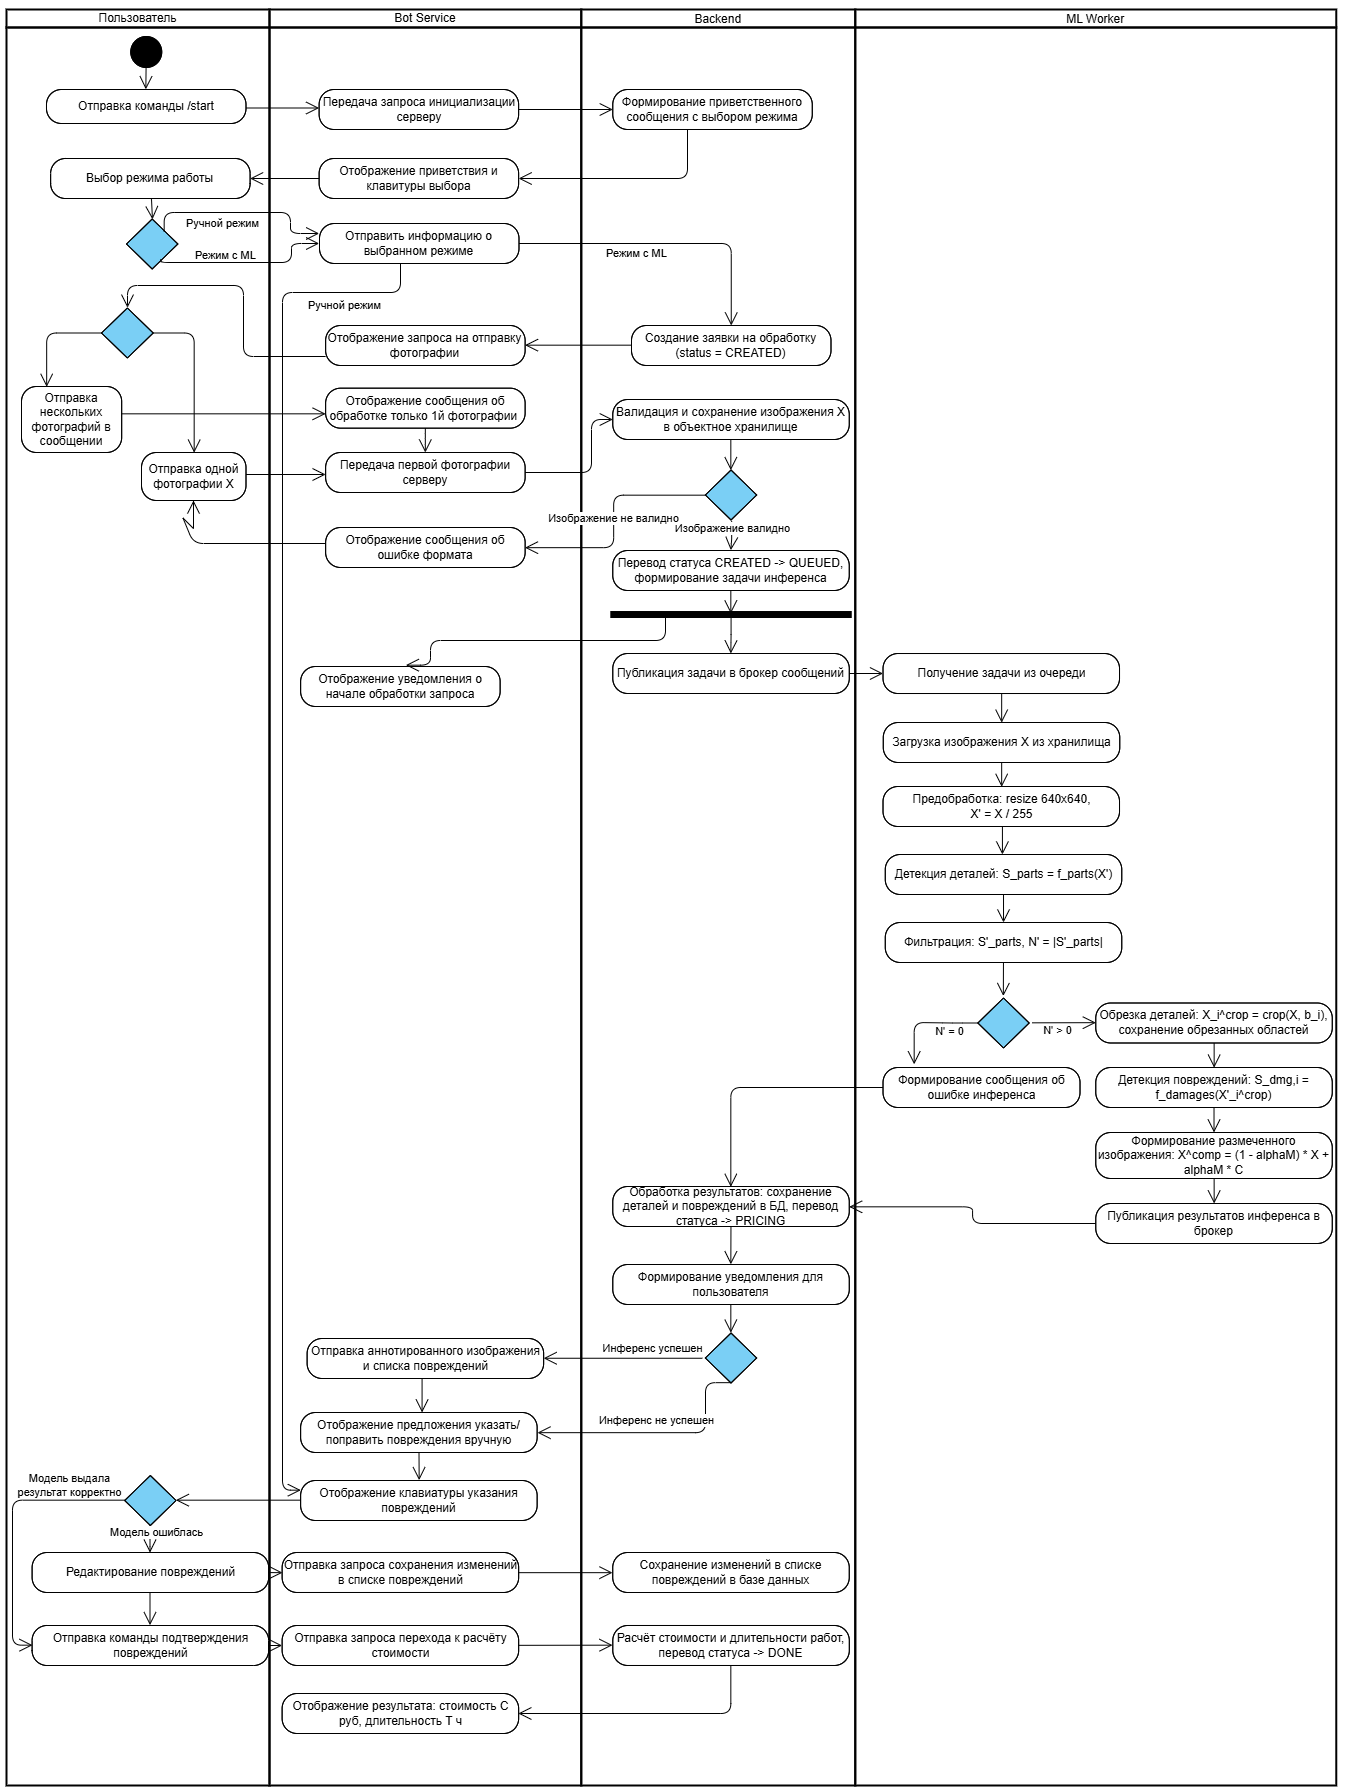
\includegraphics[scale=0.5]{UML_new}
\caption{UML Activity диаграмма сценария системы}
\end{figure}

\chapter{Программная реализация}\label{ch:7}

В данном разделе описана реализация проекта. Разработка ведётся на языке Python 3 в среде разработки Visual Studio Code для единой работы с репозиторием - все конфигурационные файлы, код и тесты располагаются в единой структуре проекта, что упрощает сопровождение. 
Компоненты системы упаковываются в Docker-контейнеры и оркестрируются с помощью Docker Compose (контейнеры: PostgreSQL, Kafka с Zookeeper, воркеры машинного обучения, бэкенд, сервис бота, nginx). Данный подход позволяет воспроизвести рабочую среду как локально на машине разработчика, так и на сервере развёртывания.

\section{Программная реализация пайплайна обучения моделей и инференса}

В рамках пайплайна анализа изображения для решения подзадач нахождения деталей и повреждений автомобиля на фотографии используется семейство моделей YOLOv8 в режиме segment через библиотеку Ultralytics. Базовые веса задаются предобученной моделью yolov8m-seg.pt, затем обучение выполняется на прикладных данных.

\begin{figure}[h]
\centering
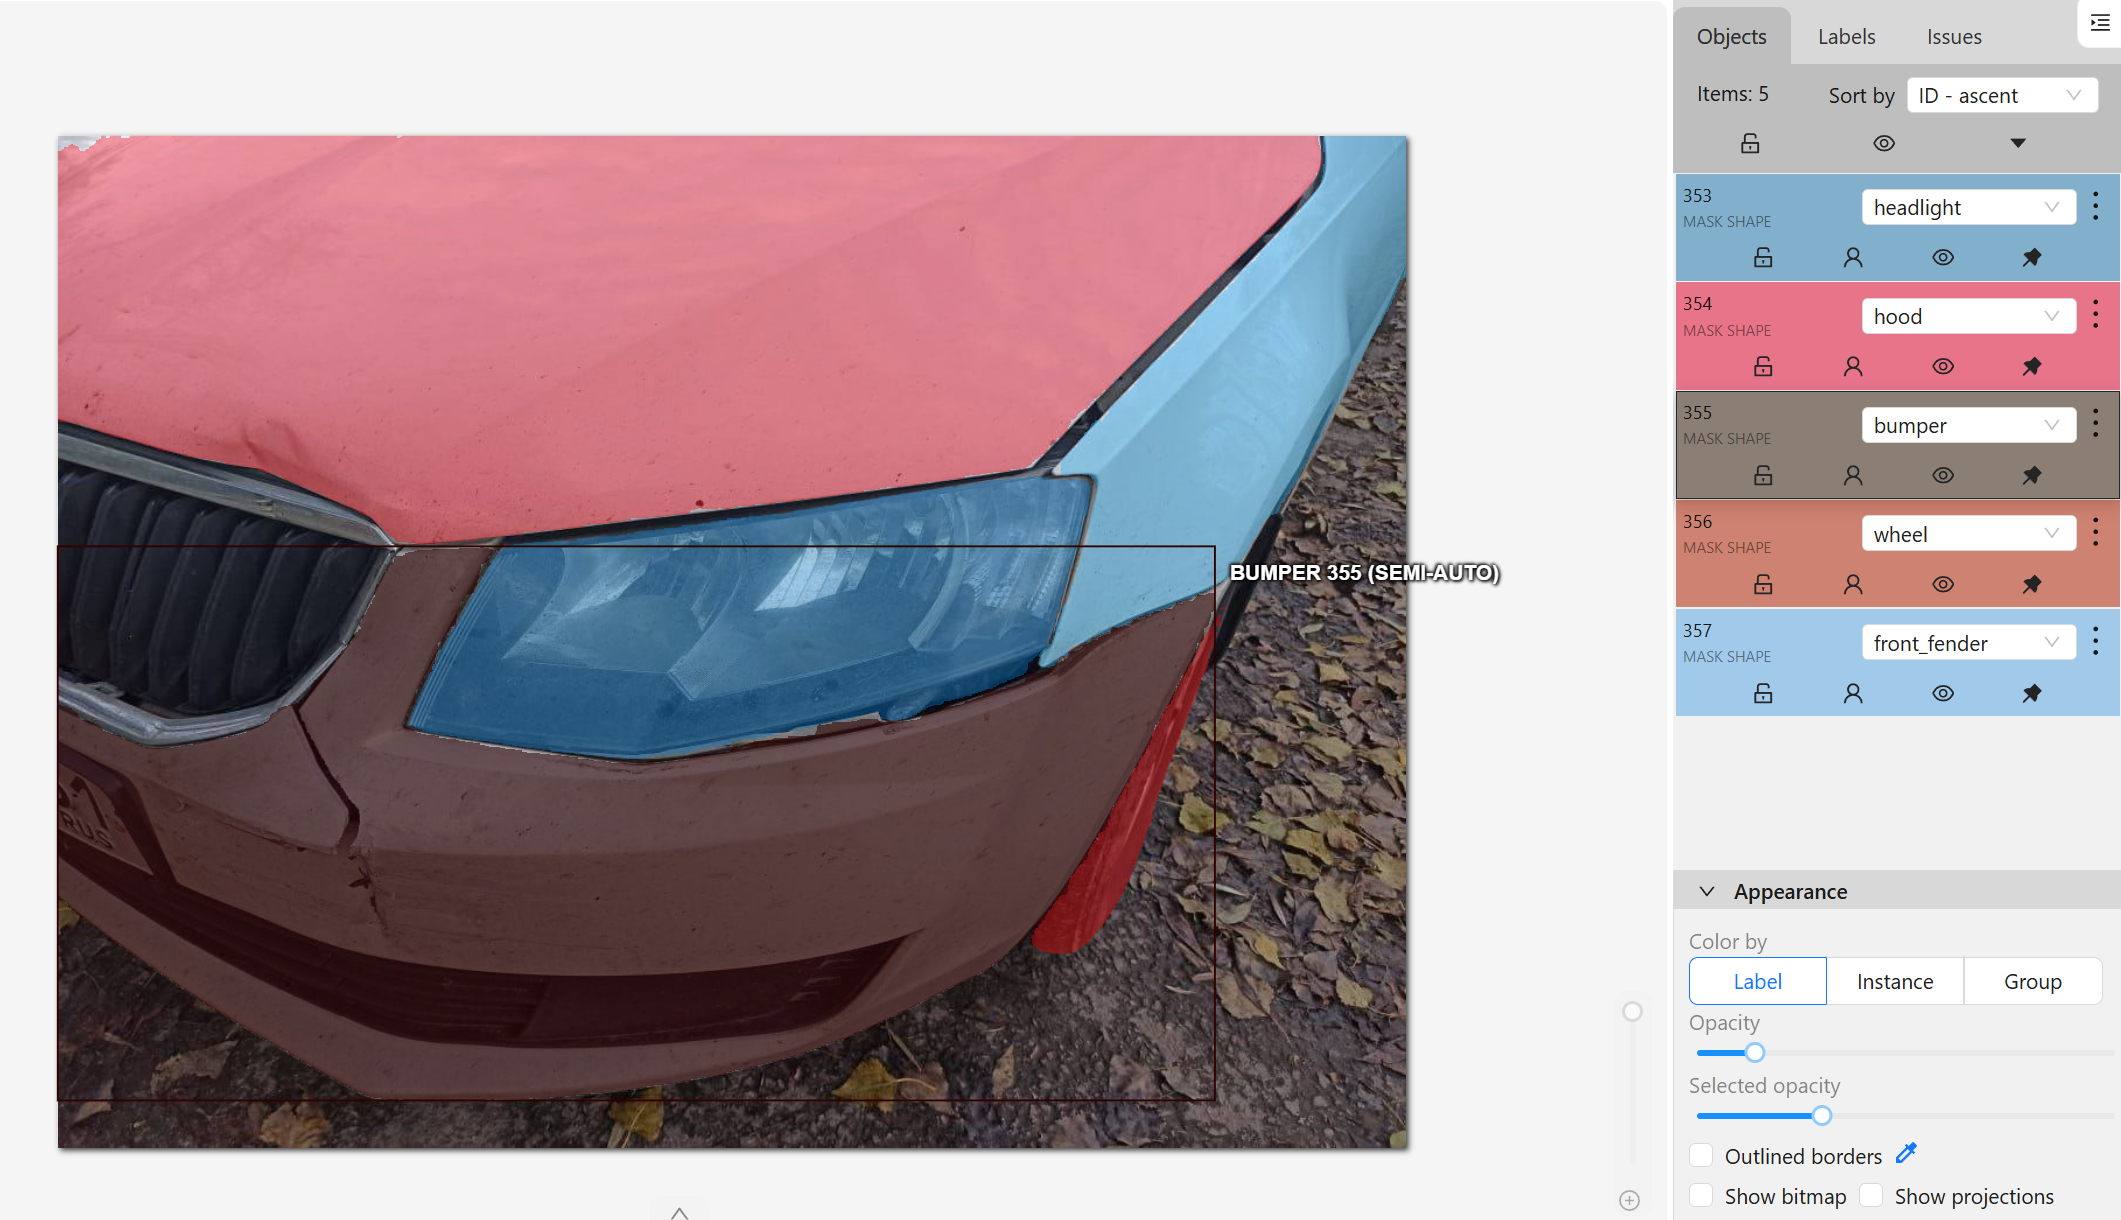
\includegraphics[scale=0.3]{details_cvat}
\caption{Пример разметки изображения для модели обнаружения деталей}
\end{figure}

Стек технологий для обучения моделей и инференса:

\begin{itemize}
    \item Python3 - реализация кода обучения и оценки
    \item Ultralytics (YOLOv8) - обучение и инференс моделей сегментации
    \item Numpy - быстрые численные операции в рамках приложения
    \item Pillow, OpenCV (opencv-python-headless) - загрузка изображений, предобработка
\end{itemize}

\begin{figure}[h]
\centering
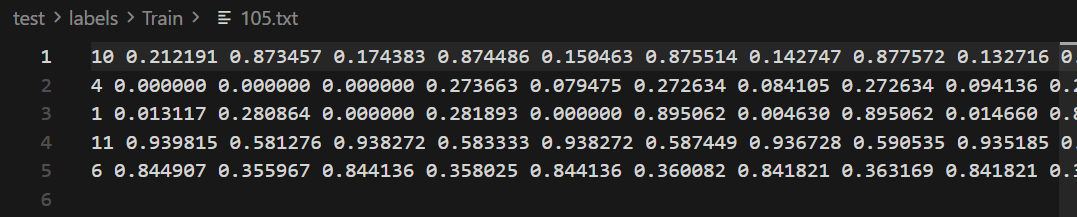
\includegraphics[scale=0.5]{train_yolo}
\caption{Пример размеченных данных}
\end{figure}

Для обучения модели обнаружения и сегментации деталей было размечено порядка 250 изображений. 
На рисунке 18 представлен пример разметки деталей автомобиля на изображении. Экспорт размеченных данных производится в формате Ultralytics YOLO Segmentation 1.0. 
На рисунке 19 показано, как выглядят размеченные данные, поступающие на вход на обучение модели. 

Каждая строка размеченных данных соответствует одному объекту и содержит идентификатор класса и последовательность нормализованных координат (x, y), описывающих контур объекта (маску). Координаты заданы в относительной системе (в диапазоне [0, 1]) относительно ширины и высоты изображения.

Аналогичная разметка была проведена для обучения модели сегментации повреждений. Для данной модели было размечено ориентировочно 370 изображений. 
Пример размеченного обрезанного изображения детали представлен на рисунке 20.

\begin{figure}[h]
\centering
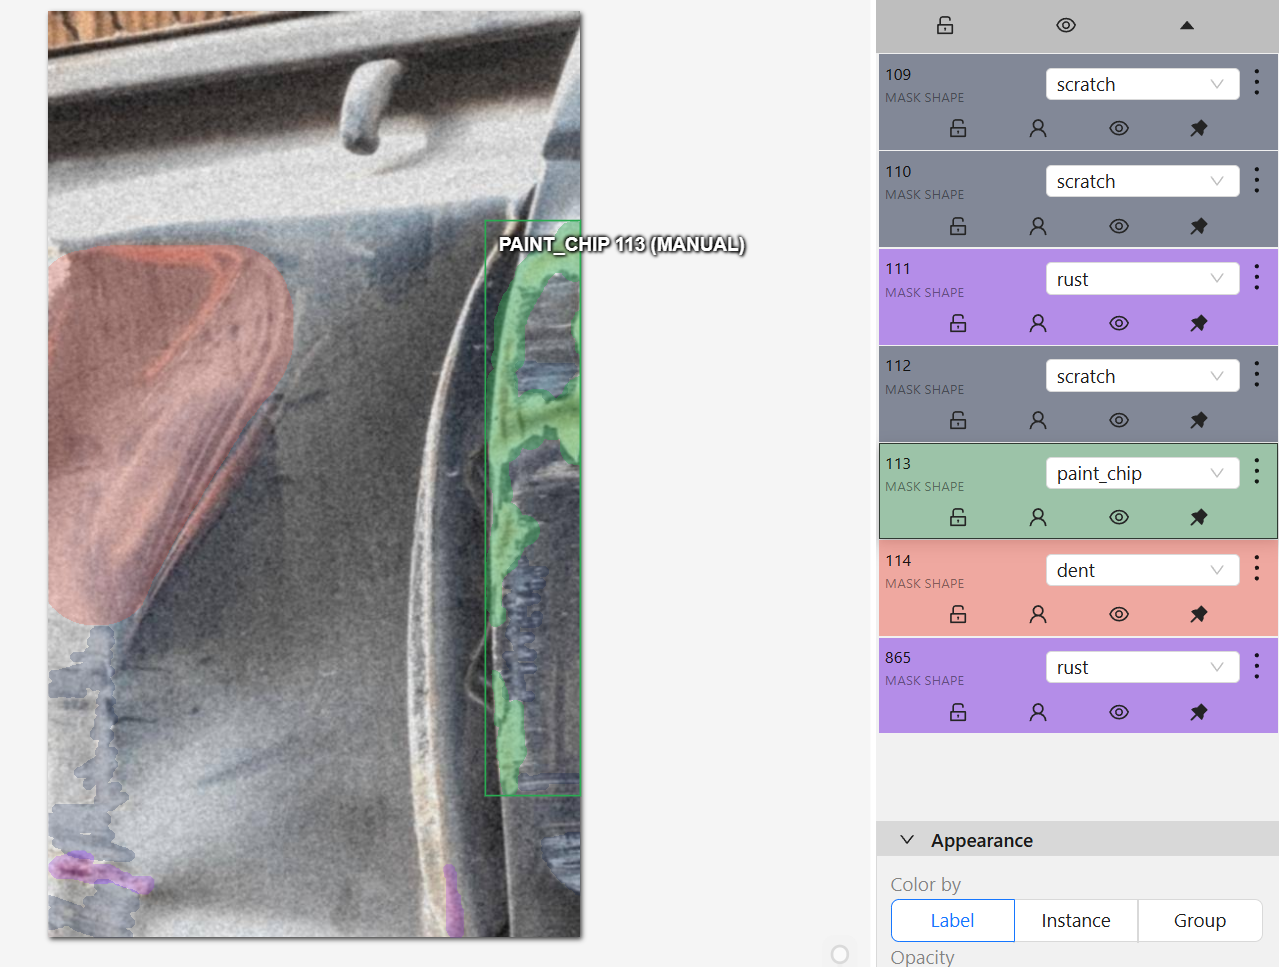
\includegraphics[scale=0.33]{damages_cvat}
\caption{Пример разметки изображения для модели обнаружения повреждений}
\end{figure}


\section{Программная реализация серверной части}

Серверная реализация строится на многослойной архитектуре и ориентирована на асинхронное выполнение. 
Стек бэкенда:
\begin{itemize}
    \item FastAPI - фреймворк для REST API
    \item uvicorn - ASGI-сервер для запуска приложения
    \item asyncio - библиотека для асинхронного выполнения кода
    \item asyncpg - для асинхронного доступа к PostgreSQL
    \item aiokafka - асинхронный клиент Apache Kafka
    \item MinIO (S3 API) - хранение исходных и аннотированных изображений
    \item Pydantic - удобная валидация данных и конфигурация (pydantic-settings)
    \item Loguru - структурированное логирование в сервисах
\end{itemize}

Реализованы и используются механизмы обеспечения отказоустойчивости и согласованности данных:
\begin{itemize}
    \item Обмен данными между бэкендом и ML-воркерами производится через топики Kafka
    \item Паттерн Transactional Outbox: фиксируются события и доставка в брокер сообщений, снимает риск рассогласования вида "запись в БД прошла, а сообщение в Kafka не дошло"
    \item Реализованы таймауты и отслеживание статусов каждой заявки
\end{itemize}


\section{Реализация интерфейса в мессенджере}

\begin{figure}[h]
\centering
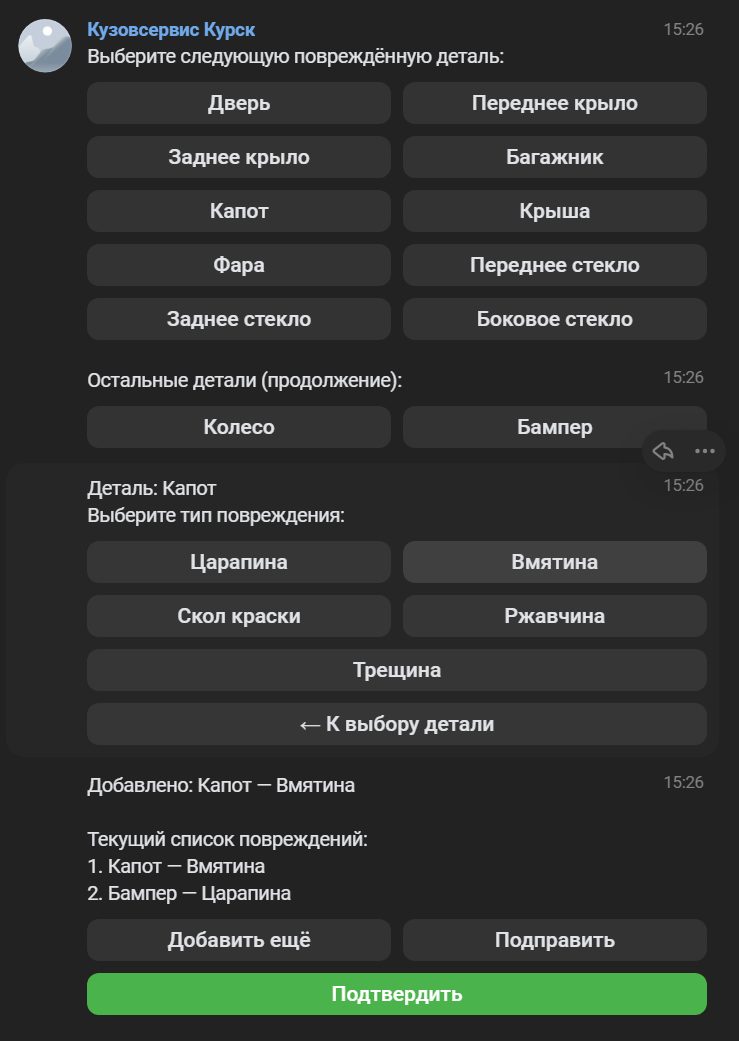
\includegraphics[scale=0.5]{interface_damages}
\caption{Интерфейс бота Вконтакте}
\end{figure}

Сценарий для пользователя реализуется в боте Вконтакте с использованием фреймворка vkbottle - асинхронный long poll, обработка сообщений и callback кнопок клавиатуры. Бот не обращается к ML напрямую, а вызывает HTTP API бэкенда и реагирует на уведомления от Kafka.

В ручном режиме ("Ручной ввод") пользователь последовательно выбирает деталь и тип повреждения, а в ML-режиме - отправляет фотографию и производится автомтаический анализ. В рамках реализации учтены ограничения платформы Вконтакте на размер и состав inline-клавиатур - длинное меню при выборе деталей разбито на несколько сообщений.



\section{Тестирование}

Функциональное и юнит-тестирование реализовано с помощью pytest и pytest-asyncio - проверяются единицы поведения доменных сервисов, сценарии бэкенда, клиент бота, генерация клавиатуры и пр. Для проверки работы кода, связанного с контроллерами (БД), используются интеграционные тесты с использованием библиотеки testcontainers, позволяющей поднять PostgreSQL в контейнере во время работы теста.

Реализована и внедрена непрерывная интеграция (CI/CD) через Github Actions - при каждом залитии новых изменений в ветку код проверяется на стиль и статический анализ (ruff, flake8 и mypy), собирается окружение и прогоняются все тесты проекта с порогом покрытия 70\%.

Также было проведено нагрузочное тестирование - написан скрипт на Python3, который отправляет более 100 запросов в секунду, содержащих изображения, для проверки отказоустойчивости системы. Фиксируются кол-во успешно обработанных сценариев, время отклика, а также другие детали работы системы, такие как, например, заполнение очереди в брокере сообщений.
\chapter{Анализ результатов}\label{ch:7}

\section{Результаты обучения моделей компьютерного зрения}

Для решения задачи автоматизированного анализа фотографии на предмет повреждений автомобиля был реализован двухэтапный ML-конвейер. Подход разделения задачи на два этапа - поиска деталей и поиска повреждений - позволил устранить проблему логически некорректных сочетаний (например, <фара - спущенная шина>), а также приблизить модель к реальному сценарию работы автосервиса, где модель, как и человек, анализирует повреждения в рамках отдельных деталей автомобиля.

В ходе работы были обучены две модели компьютерного зрения на базе YOLOv8-seg:

\begin{itemize}
    \item Модель сегментации деталей автомобиля
    \item Модель сегментации повреждений автомобиля
\end{itemize}


\begin{table}[H]
\centering
\caption{Итоговые метрики модели сегментации деталей}
\begin{tabular}{|l|l|}
\hline
\textbf{Метрика} & \textbf{Значение} \\
\hline
Размер обучающей выборки     & 174 изображения \\
\hline
Размер валидационной выборки & 26 изображений \\
\hline
Размер тестовой выборки      & 26 изображений \\
\hline
Precision (Box)              & 0.766 \\
\hline
Recall (Box)                 & 0.517 \\
\hline
mAP@0.5 (Box)                & 0.560 \\
\hline
mAP@0.5:0.95 (Box)           & 0.471 \\
\hline
Начальный box\_loss          & 1.171 \\
\hline
Конечный box\_loss           & 0.3387 \\
\hline
Количество итераций (эпох)   & 150 \\
\hline
\% падения loss              & 346\% \\
\hline
\end{tabular}
\end{table}

\begin{table}[H]
\centering
\caption{Итоговые метрики модели сегментации повреждений}
\begin{tabular}{|l|l|}
\hline
\textbf{Метрика} & \textbf{Значение} \\
\hline
Размер обучающей выборки     & 313 изображений \\
\hline
Размер валидационной выборки & 29 изображений \\
\hline
Размер тестовой выборки      & 30 изображений \\
\hline
Precision (Mask)             & 0.684 \\
\hline
Recall (Mask)                & 0.449 \\
\hline
mAP@0.5 (Mask)               & 0.474 \\
\hline
mAP@0.5:0.95 (Mask)          & 0.307 \\
\hline
Начальный seg\_loss          & 3.463 \\
\hline
Конечный seg\_loss           & 1.377 \\
\hline
Количество итераций          & 137 (137/150 EarlyStopping) \\
\hline
\% падения loss              & 251\% \\
\hline
\end{tabular}
\end{table}

Результаты обучения обеих моделей визуализированы и представлены на графиках.
На рисунках 22 и 23 представлены графики loss и метрик, а на рисунках 24 и 25 - скриншоты процессов обучения моделей.


\begin{figure}[H]
\centering
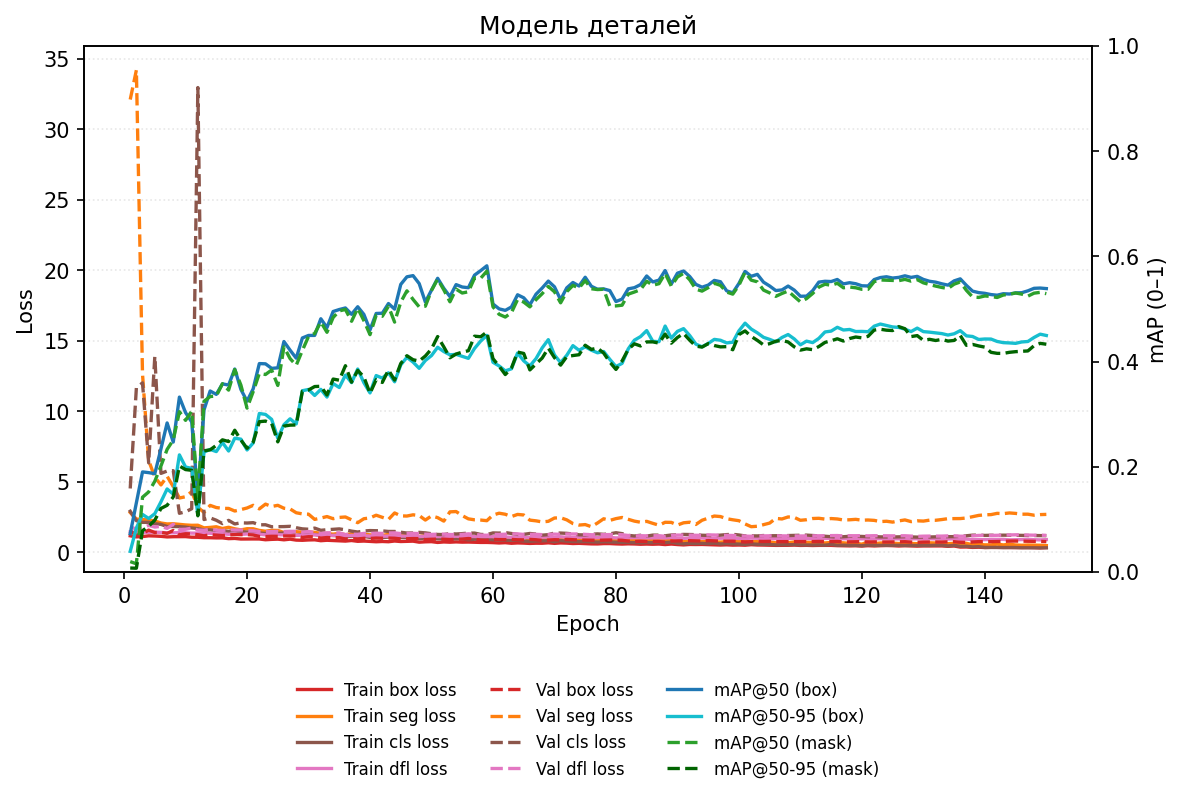
\includegraphics[scale=0.8]{details_training_combined}
\caption{График метрик обучения модели деталей}
\end{figure}

\begin{figure}[H]
\centering
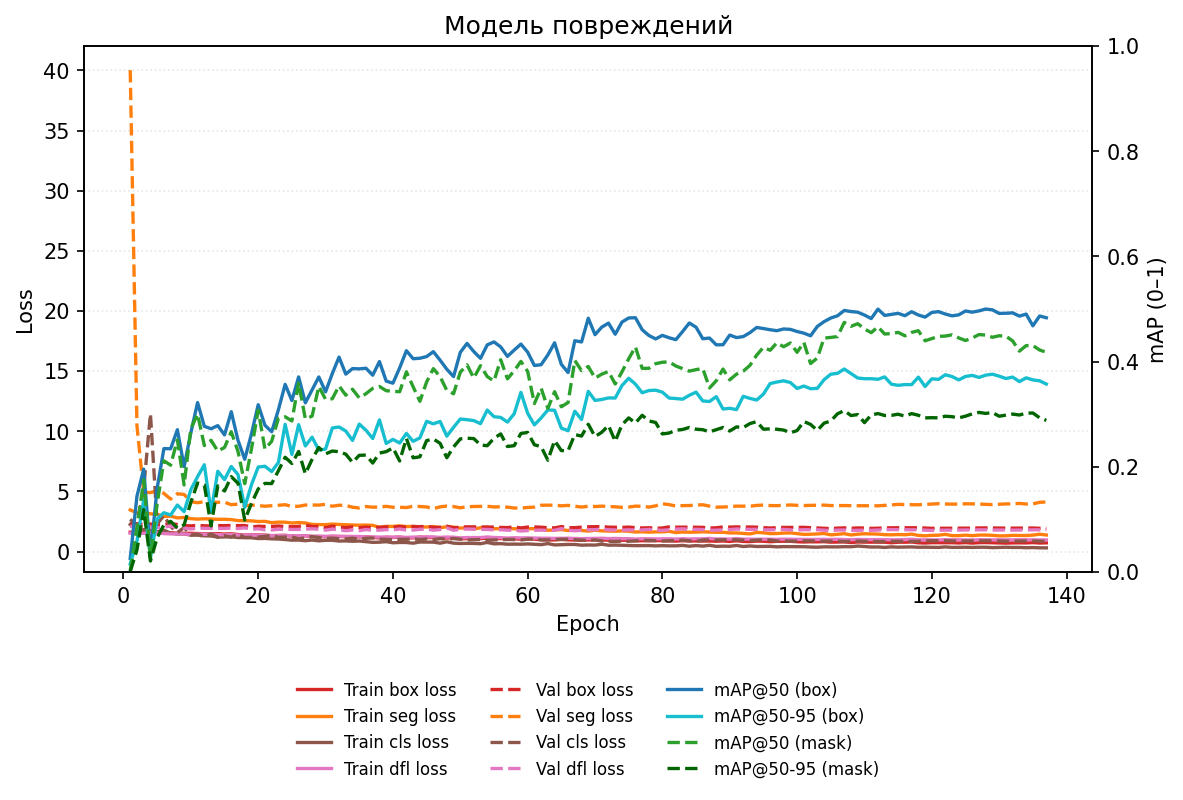
\includegraphics[scale=0.8]{damages_training_combined}
\caption{График метрик обучения модели повреждений}
\end{figure}

\begin{figure}[H]
\centering
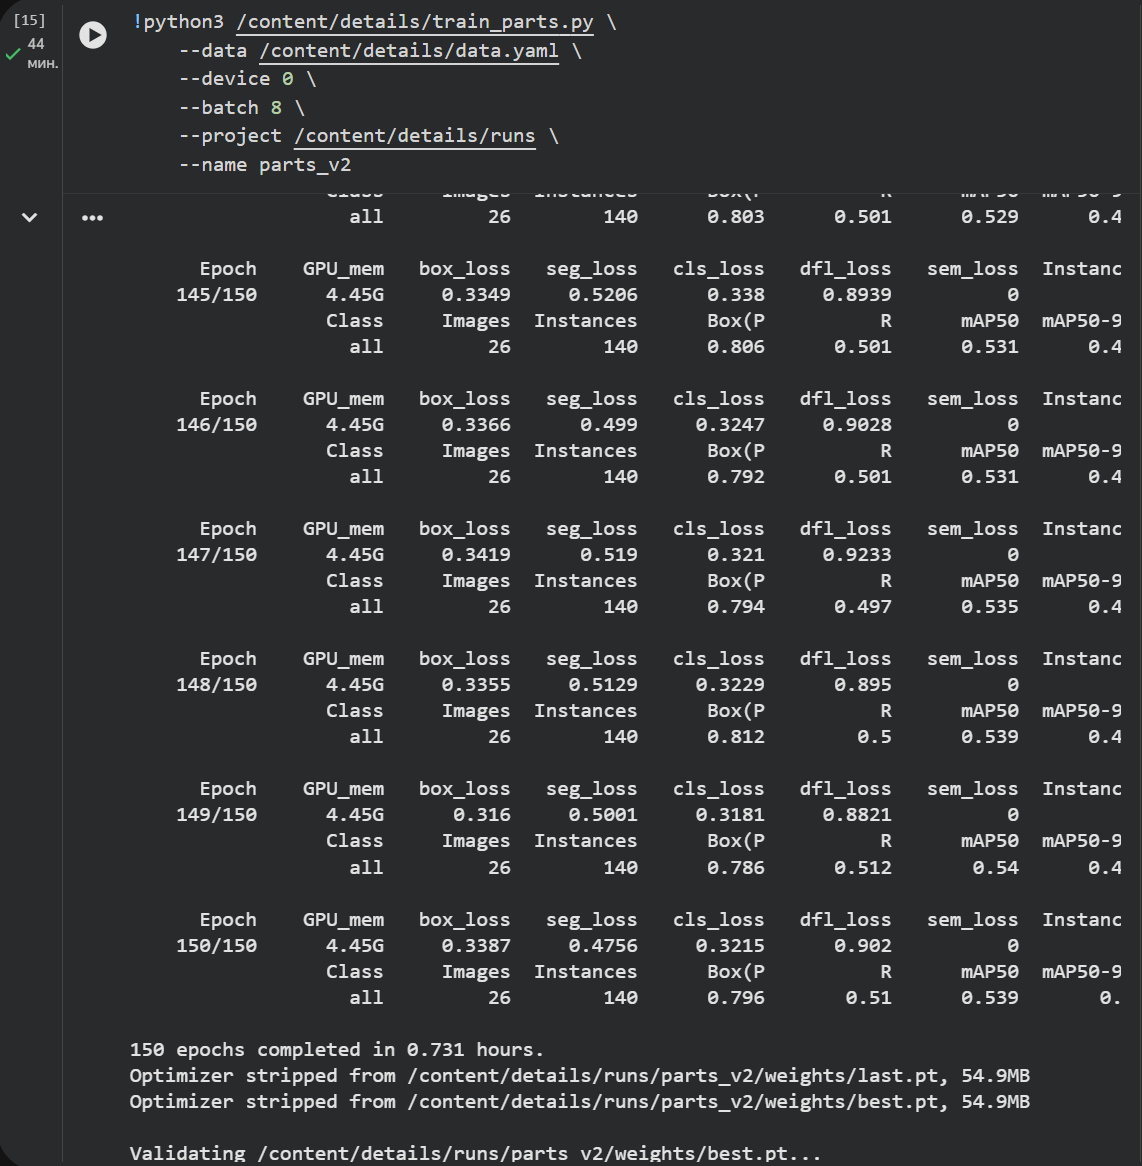
\includegraphics[scale=0.4]{details_training}
\caption{Скриншот процесса обучения модели деталей}
\end{figure}

\begin{figure}[H]
\centering
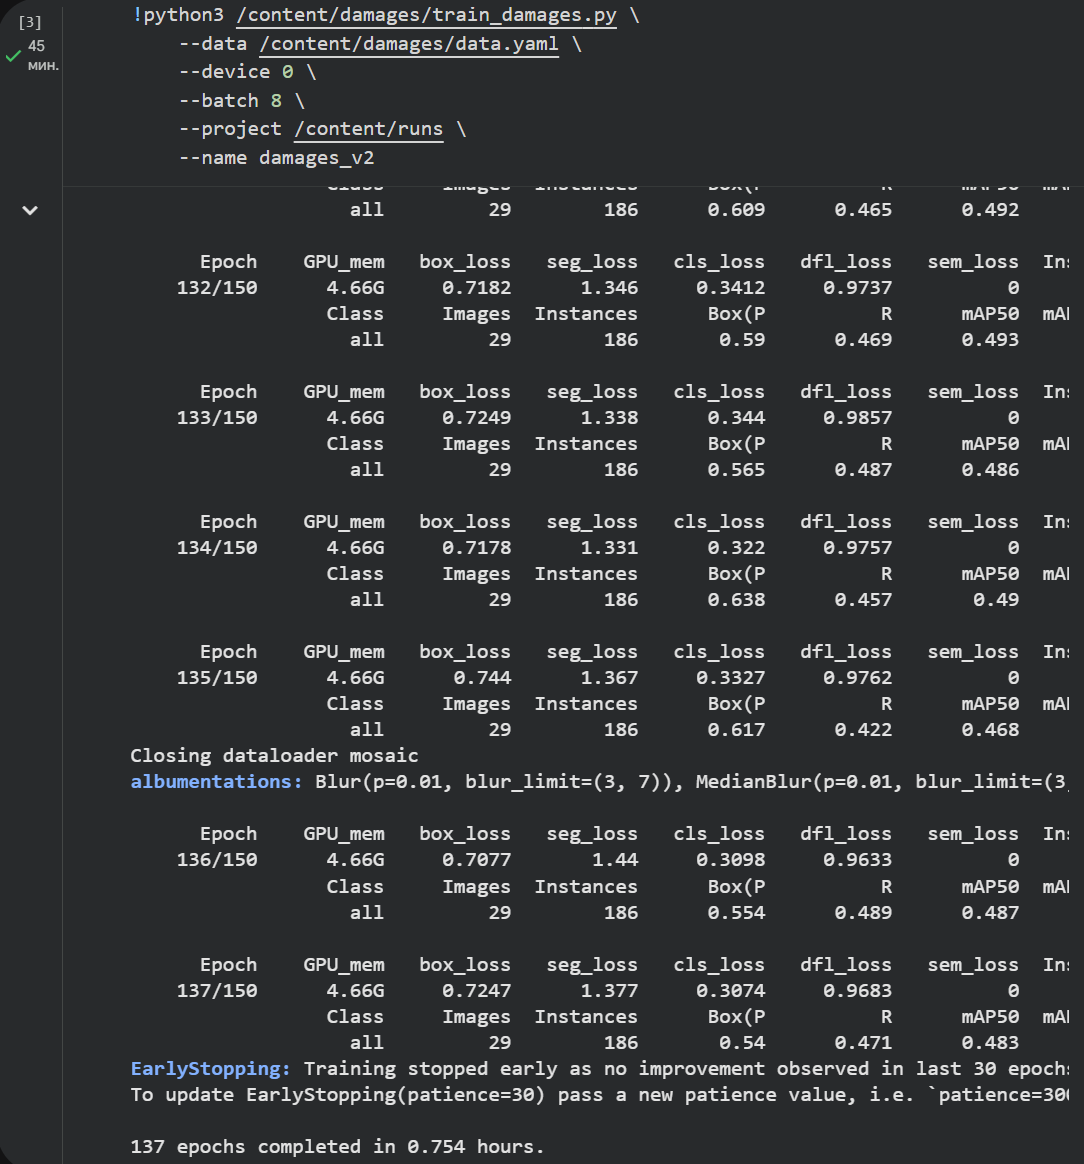
\includegraphics[scale=0.4]{damages_training}
\caption{Скриншот процесса обучения модели повреждений}
\end{figure}

По полученным графикам можно сделать вывод о том, что модели демонстрируют сходимость в ходе обучения (снижение loss - усвоение закономерностей). Не менее показательными при этом являются не только значения функции потерь, но и итоговые значения precision, recall и mAP на валидационной и тестовой выборках (таблицы 7 и 8) - именно они показывают пригодность моделей к задаче.

Если сравнивать результаты двух моделей, то модель сегментации деталей демонстрирует результаты лучше, чем модель сегментации повреждений. Это объясняется рядом причин:
\begin{itemize}
    \item Автомобильные детали намного крупнее и имеют в большинстве случаев схожую форму
    \item Повреждения более вариативны по форме, размеру, степени выраженности и условиям съёмки
\end{itemize}

По этой причине задача сегментации повреждений является намного более сложной, а метрики по ней закономерно ниже.

С практической точки зрения сервис сохраняет прикладную ценность даже в случае неполного или неидеального распознавания - пользователь имеет возможность отредактировать результат и получить расчёт стоимости. Таким образом, ML-модели позволяют сократить объём ручной работы, но не выступают как полностью необратимая система принятия решений.

Важным результатом является визуальная интерпретируемость работы моделей. В конце работы пользователю возвращается аннотированное изображение с наложенными масками повреждений (рисунок 28), что позволяет оценить корректность работы модели. Это повышает доверие к сервису и облегчает проверку результата человеком.

На рисунках 26-30 представлены результаты работы моделей деталей и повреждений - аннотированные изображения.

\begin{figure}[H]
\centering
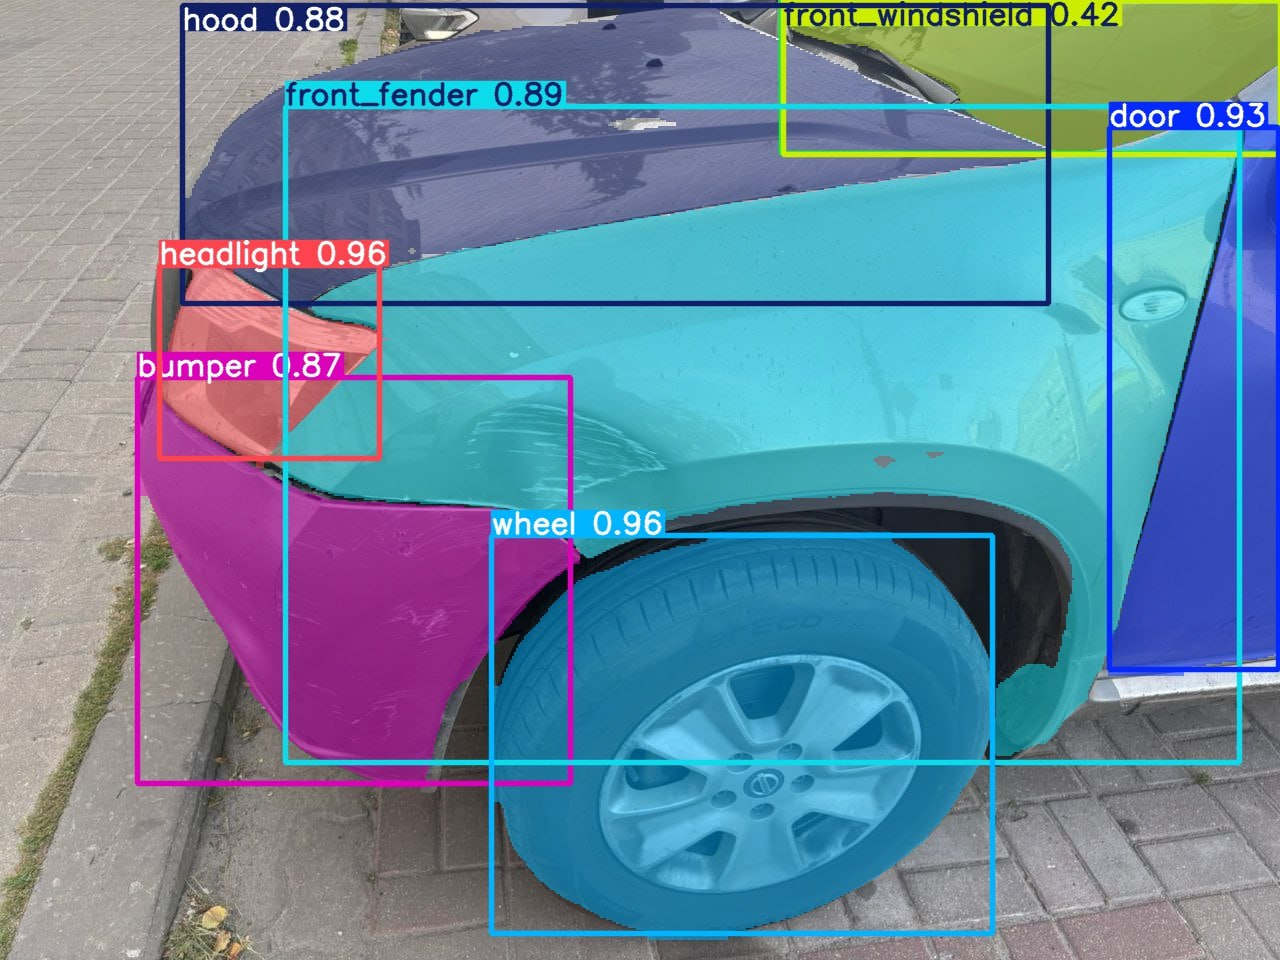
\includegraphics[scale=0.35]{details_inference_example}
\caption{Пример сегментации деталей на исходной фотографии}
\end{figure}

\begin{figure}[H]
\centering
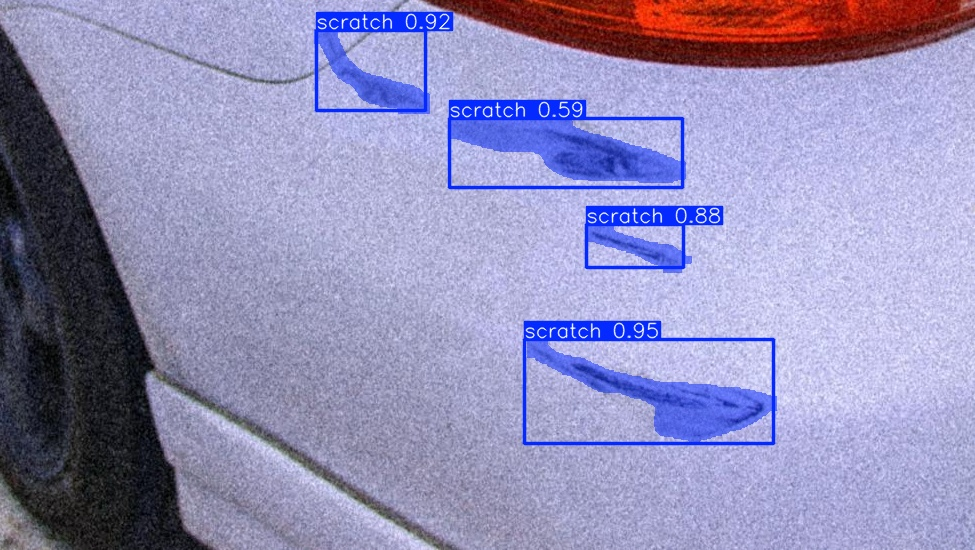
\includegraphics[scale=0.4]{damages_inference_example}
\caption{Пример сегментации повреждений на обрезанных фрагментах деталей}
\end{figure}

\begin{figure}[H]
\centering
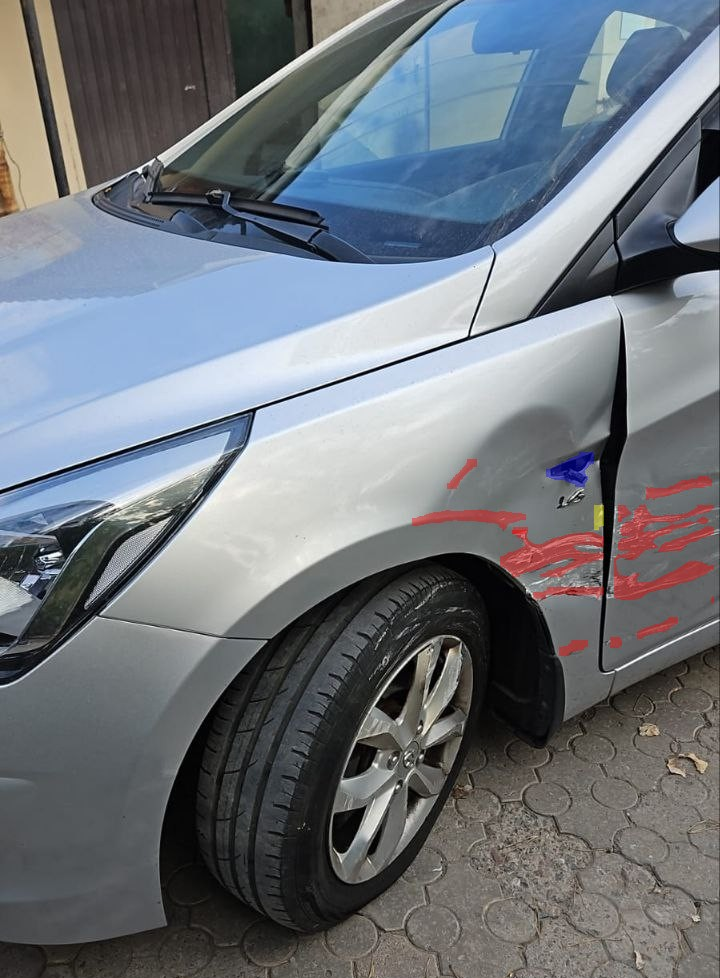
\includegraphics[scale=0.4]{annotated_user_image}
\caption{Пример итогового аннотированного изображения, отправляемого пользователю}
\end{figure}

\begin{figure}[H]
\centering
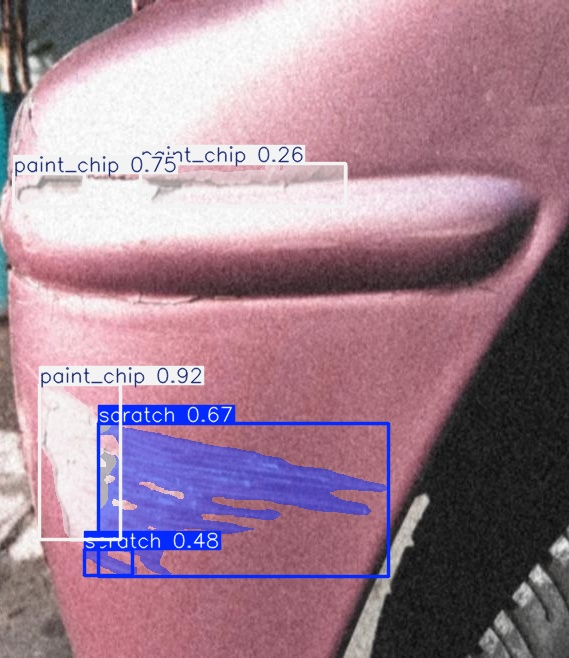
\includegraphics[scale=0.5]{many_damages_inference}
\caption{Пример корректного определения нескольких типов повреждений}
\end{figure}

\begin{figure}[H]
\centering
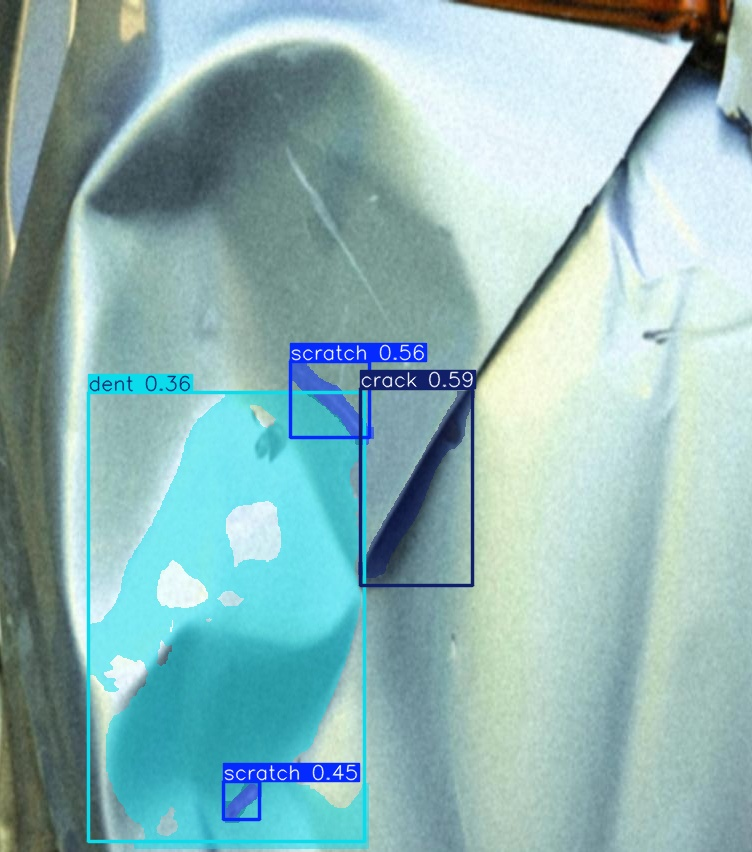
\includegraphics[scale=0.3]{damages_not_nice_inference}
\caption{Пример частично ошибочного определения, демонстрирующий ограничения модели}
\end{figure}

Анализируя полученные результаты, можно выделить ряд причин, по которым результат некоторых предсказаний может не соответствовать реальным повреждениям:
\begin{enumerate}[label=\arabic*.]
    \item Ограничен объём датасета и размеченных фотографий
    \item Дисбаланс классов - есть типы повреждений, которые встречаются намного реже частых, таких как царапины
    \item Сложность самих визуальных объектов, в особенности мелких царапин или вмятин
    \item Неоднозначность границ повреждений при разметке
\end{enumerate}

Достигнутый результат по ML-части можно оценить как достаточный для задачи предварительной автоматизированной оценки, но требует дальнейшего улучшения за счет увеличения кол-ва различных размеченных фотографий, в особенности, повреждений.




\section{Результаты нагрузочного тестирования}

\begin{table}[h!]
\centering
\resizebox{1.05\textwidth}{!}{
\begin{tabular}{|c|c|c|c|c|c|}
\hline
\textbf{Целевая нагрузка} & \textbf{Успешность} & \textbf{Наблюдаемый RPS} & \textbf{p50 полного цикла} & \textbf{p95 полного цикла} & \textbf{Ошибки} \\
\hline
50 RPS  & 100\%  & 37.04 RPS & 1.58 с  & 2.12 с  & - \\
\hline
120 RPS & 100\%  & 33.28 RPS & 4.40 с  & 5.62 с  & - \\
\hline
200 RPS & 93.34\% & 21.77 RPS & 12.32 с & 14.93 с & 130x ReadError \\
\hline
\end{tabular}
}
\caption{Результаты нагрузочного тестирования}
\end{table}

Нагрузочное тестирование проводилось для полного ML-сценария: создание заявки, загрузка изображения в S3-хранилище и постановка задачи инференса в Kafka. Его результаты представлены в таблице 9. При нагрузках 50 и 120 RPS обработка всех запросов прошла без ошибок. Это подтверждает устойчивость системы при повышенной нагрузке: все микросервисы работали штатно на протяжении тестирования.

На текущем одноузловом стенде система упирается примерно в 33–37 RPS. При попытке подать нагрузку выше этого значения система не выдаёт ошибок, но растёт задержка: p95 увеличивается с 2.12 с до 5.62 с.

При 200 RPS начинается деградация: успешность запросов снижается до 93.34\%, а p95 достигает почти 15 секунд. Это показывает практический предел текущего локального стенда. Основная причина ограничения - запуск backend в одном uvicorn-процессе и размещение всех сервисов на одной машине.

Итог: система выдерживает стабильную обработку около 35 RPS без ошибок, корректно буферизует ML-задачи через Kafka и показывает устойчивость при умеренной перегрузке. Для достижения уровня выше 100 RPS в продуктиве требуется горизонтальное масштабирование backend-сервиса и ML worker'ов.




\section{Результаты работы сервиса}

Пользователь взаимодействует с сервисом через бот в мессенджере Вконтакте. По итогам реализации сервис поддерживает 2 режима работы - автоматический с анализом фотографии и ручной режим ввода повреждений. 

Пользовательский сценарий начинается с команды /start (или нажатия кнопки "Начать") с последующим выбором режима работы (Рисунок 31). При выборе режима с фотографией пользователь отправляет изображение автомобиля с видимым повреждением (Рисунок 32). 

\begin{figure}[H]
\centering
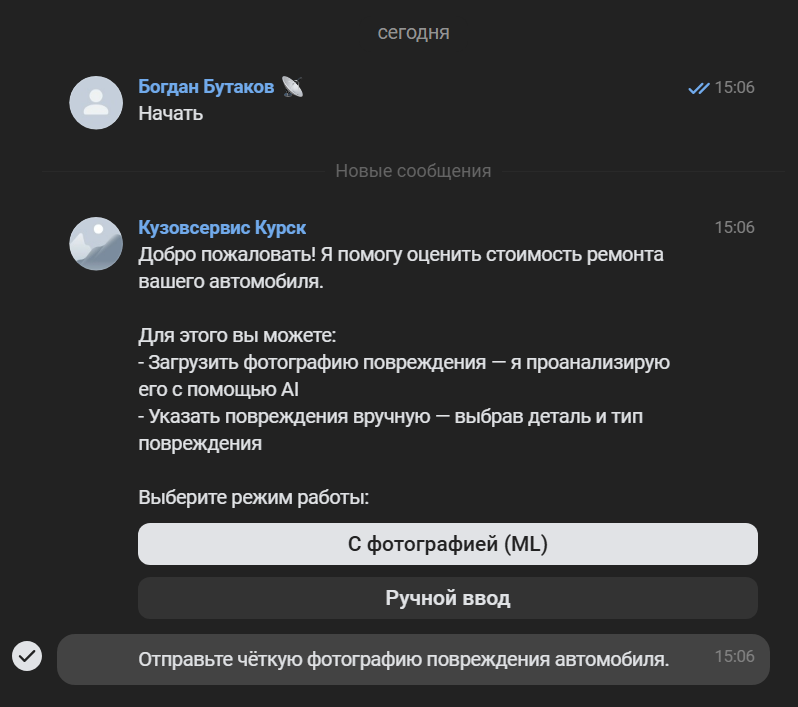
\includegraphics[scale=0.55]{start_interface}
\caption{Интерфейс бота (начальный этап выбора режима работы)}
\end{figure}

\begin{figure}[H]
\centering
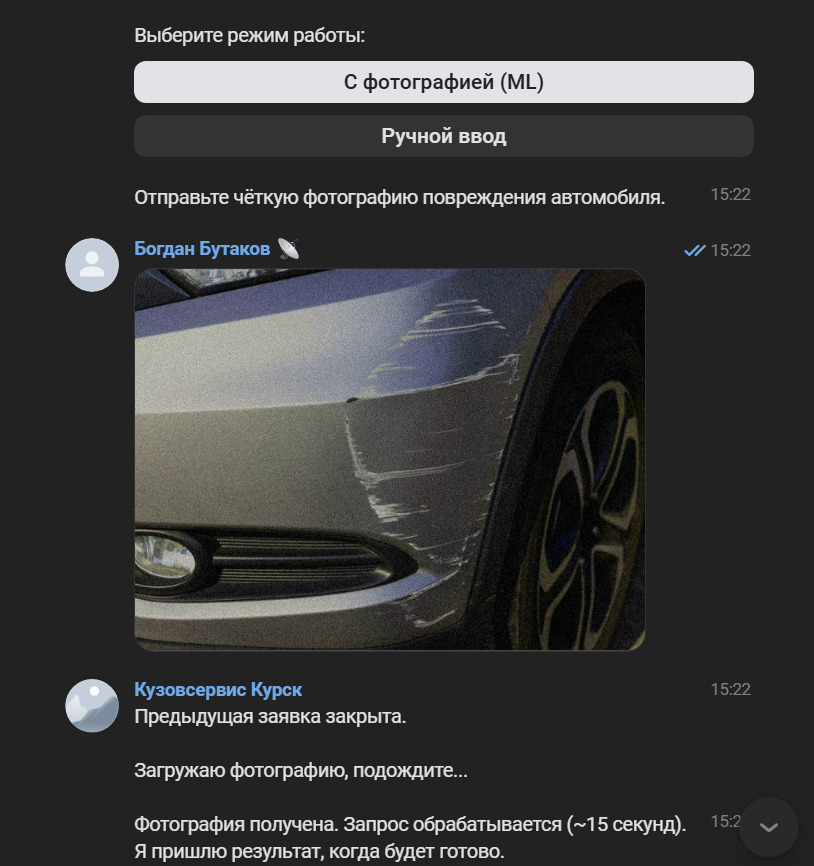
\includegraphics[scale=0.75]{ml_mode_interface}
\caption{Пример взаимодействия с ботом в режиме ML}
\end{figure}

Сервис сохраняет фотографию, после чего система выполняет обработку изображения и возвращает аннотированное изображение вместе со списком найденных повреждений и клавиатуру с возможностью отредактировать повреждения и кнопкой подтверждения (Рисунок 33).

\begin{figure}[H]
\centering
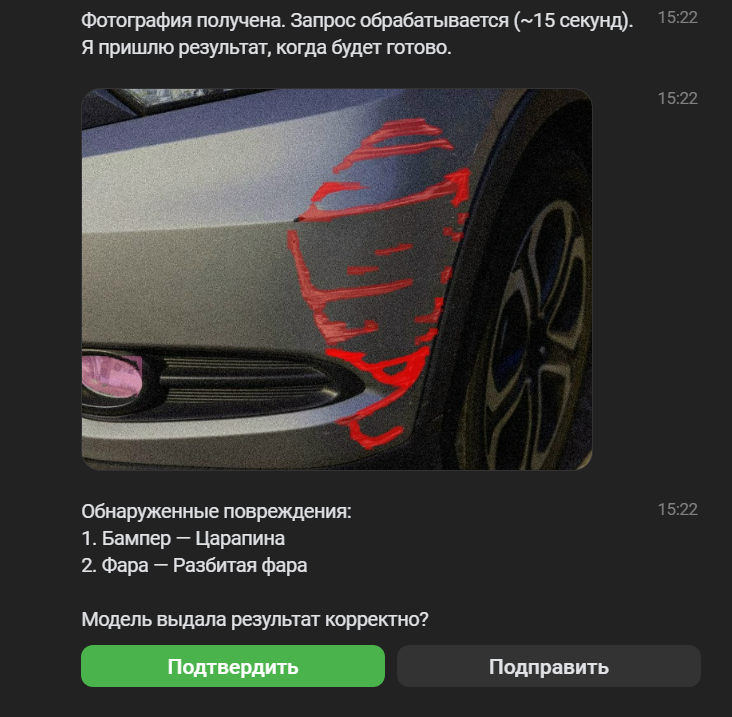
\includegraphics[scale=0.8]{ml_mode_result}
\caption{Результат обработки фотографии в режиме ML}
\end{figure}

Существенным преимуществом в интерфейсе бота является функционал, где при необходимости пользователь может отредактировать список обнаруженных повреждений - удалить, изменить тип найденного повреждения или его принадлежность к детали, или добавить необнаруженное повреждение (Рисунки 34 и 35). Это делает систему более пригодной для практического пользования и не делает пользователя зависимым от возможных просчётов модели.

\begin{figure}[H]
\centering
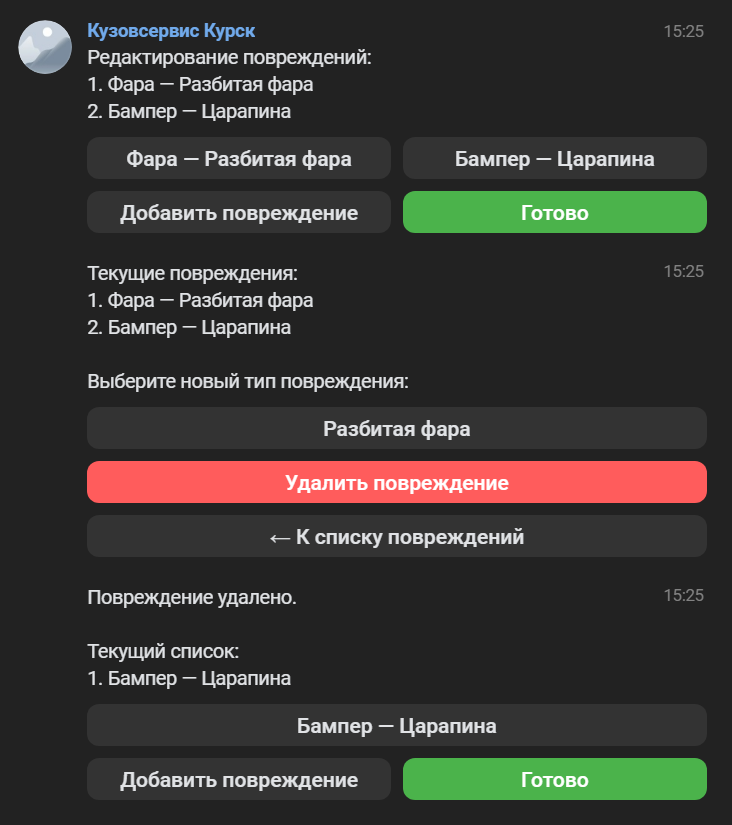
\includegraphics[scale=0.85]{delete_damage}
\caption{Редактирование списка повреждений (удаление)}
\end{figure}

\begin{figure}[H]
\centering
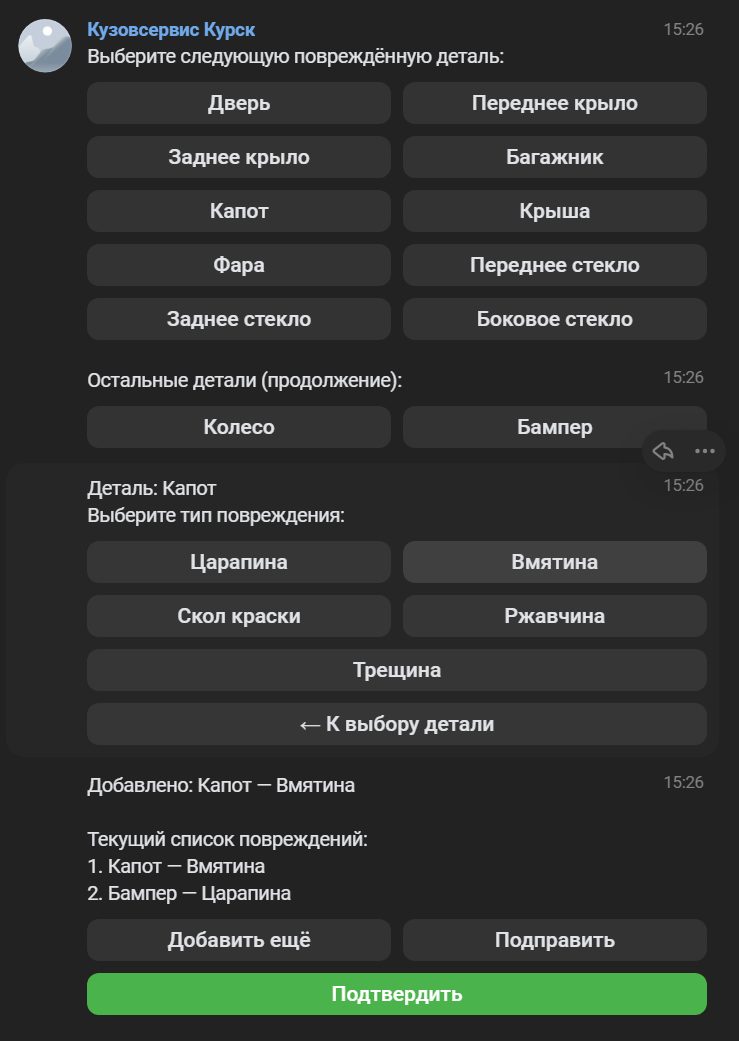
\includegraphics[scale=0.85]{interface_damages}
\caption{Редактирование списка повреждений (добавление)}
\end{figure}

После того, как пользователь введёт полный список повреждений, он может нажать кнопку "Подтвердить", и сервис сразу выдаст полную стоимость и длительность работ в рабочих часах (Рисунок 36):

\begin{figure}[H]
\centering
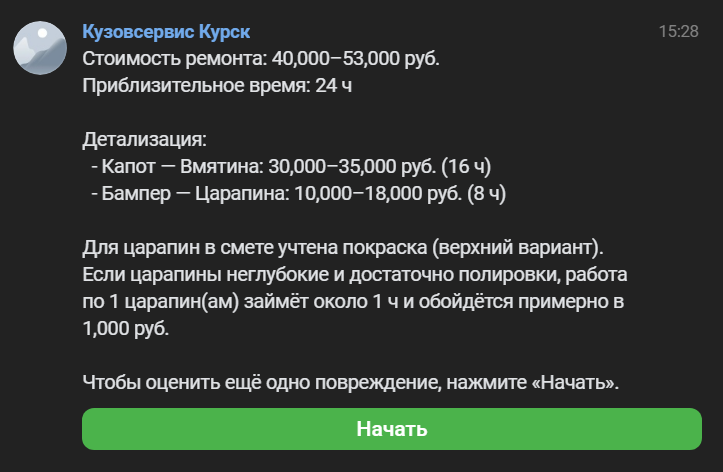
\includegraphics[scale=0.85]{price_result}
\caption{Результат подсчёта стоимости и длительности работ}
\end{figure}

Пользователь может выбрать и режим ручного ввода повреждений. В этом режиме ему доступен схожий функционал, что и в режиме ML при редактировании повреждений, только теперь пользователь вводит все повреждения с нуля самостоятельно. (Рисунок 37)

\begin{figure}[H]
\centering
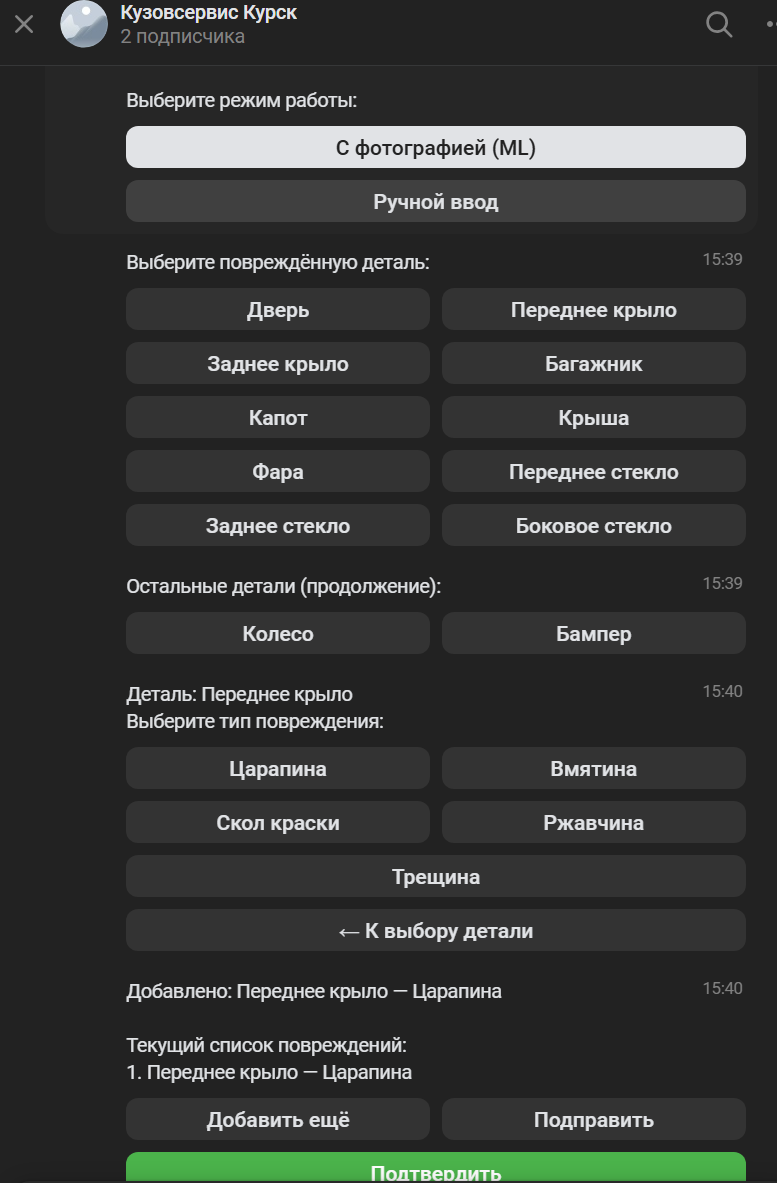
\includegraphics[scale=0.8]{manual_mode}
\caption{Пример взаимодействия с ботом в ручном режиме}
\end{figure}

Таким образом, с точки зрения пользовательского опыта достигнут результат, при котором:
\begin{itemize}
    \item Сценарий запуска является быстрым и понятным
    \item Доступна свобода действий и выбора автоматического и ручного режима
    \item Пользователь имеет удобный, не перегруженный интерфейс и может контролировать результат
    \item Итоговая смета представляется в понятном виде
\end{itemize}

\section{Оценка выполнения задач исследования}

В рамках работы был подготовлен датасет изображений деталей и повреждений и выполнена разметка в формате, пригодном для дообучения моделей YOLOv8-seg. Уровень решения задачи можно оценить как высокий с точки зрения работоспособного датасета и средний с точки зрения охвата всех редких случаев. Ограничением всё так же остаётся необходимости дальнейшего расширения и балансировки выборки, особенно для сложных и трудноразличимых повреждений.

Разработка модулей для обработки изображений также решена. На этапе обучения используется конфигурируемый набор аугментаций, что позволило модели быть устойчивой к разнообразию фотографий. Использование аугментаций также помогло частично компенсировать ограниченный объём размеченных данных. 
Недостатки съёмки, такие как нечёткие фотографии, блики, плохое освещение, всё же существенно снижают качество распознавания, так как учесть все возможные вариации съёмки и передать эту информацию модели невозможно. 
Однако обучение моделей показало, что они демонстрируют сходимость в ходе обучения, что видно по функции потерь и метрикам - это означает, что модели пригодны к задаче, и главной проблемой является необходимость большого количества грамотно размеченных данных. 

Бизнес-логика оценки стоимости и длительности ремонта реализована в полном объёме. Система корректно учитывает все особенности предметной области и обладает знанием о всех расценках автосервиса и корректно применяет их ко всем парам деталей и повреждений, как это делают сотрудники автосервиса. 

Система построена в виде микросервисной архитектуры, включающей Backend API, Bot Service и ML Worker. Обмен сообщениями осуществляется через Kafka, для хранения изображений используется S3, а данные заявок и повреждений сохраняются в PostgreSQL.  Такое архитектурное решение позволило разделить ответственность между разными компонентами системы, сделать её масштабируемой. Интеграция с ботом в мессенджере выполнена - пользователь может полностью пройти весь сценарий оценки, не покидая интерфейс Вконтакте.
Архитектура базы данных соответствует микросервисному подходу и поддерживает основные сценарии работы системы.

Также произведена интеграция CI/CD - настроен конвейер с использованием GitHub Actions, выполняющий автоматическую проверку стиля кода и запуск тестов при изменениях в целевой ветви. Система контейнеризирована с использованием Docker Compose, что обеспечивает воспроизводимую локальную сборку, и развёрнута на сервере.

Проведено полноценное тестирование работоспособности системы - в проекте реализовано более 500 юнит- и интеграционных тестов, которые поддерживают устойчивость реализованных сценариев на уровне кода. 
Дополнительно реализован отдельный скрипт нагрузочного тестирования, имитирующий полный сценарий ML режима работы: создание заявки, загрузка изображений в объектное хранилище. Это позволило оценить пропускную способность системы и устойчивость к интенсивному потоку запросов. Результаты нагрузочного тестирования были представлены выше в таблице 9.

На основании приведённого анализа можно сделать вывод о том, что все поставленные задачи получили практическое решение. Наибольший потенциал для дальнейшего улучшения остаётся в повышении качества ML-моделей и разметки большего количества фотографий деталей и повреждений.

Следует отметить, что достигнутый результат не означает полной замены эксперта-оценщика. Итоговая система является инструментом предварительной автоматизированной оценки, а не окончательным юридически значимым подсчётом стоимости ремонта.




% Заключение
\cchapter{ЗАКЛЮЧЕНИЕ}                       % Заголовок
\addcontentsline{toc}{chapter}{ЗАКЛЮЧЕНИЕ}  % Добавляем его в оглавление

Данная работа позволила достигнуть поставленной цели - повышения эффективности процесса оценки стоимости ремонта поврежденных автомобилей. Достижение данной цели оценивалось по двум основным факторам:
\begin{enumerate}[label=\arabic*.]
  \item Производительность системы
  \item Минимизация человеческого участия
\end{enumerate}

\begin{table}[h!]
\centering
\begin{tabular}{|p{5cm}|p{3cm}|p{5cm}|p{3cm}|}
\hline
\textbf{Критерий} & \textbf{Исходное состояние} & \textbf{Результат после внедрения} & \textbf{Вывод} \\
\hline
Скорость получения предварительной сметы и длительности работ & 30 минут & 1 минута & Значительно сократилась \\
\hline
Возможность параллельной обработки обращений & Ограниченная & Есть за счет микросервисной архитектуры и очередей & Цель достигнута \\
\hline
Надежность и воспроизводимость сценария & Зависела от сотрудника & Формализована в виде системы и тестов & Цель достигнута \\
\hline
\end{tabular}
\caption{Сравнение состояния до и после внедрения системы}
\end{table}

С точки зрения производительности разработанный сервис обеспечивает автоматизированное прохождение сценария обработки обращения. Полученные в нагрузочном тестировании значения по пропускной способности и времени отклика показывают, что система способна выдержать поток обращений на уровне не менее 120 RPS и оставаться отказоустойчивой. Следовательно, первый критерий достижения цели можно считать выполненным.

С точки зрения минимизации человеческого участия цель также достигнута. В разработанном сервисе пользователь получает предварительный результат автоматически, и сотруднику автосервиса не требуется тратить время и отвлекаться на согласования и переписку с клиентом. Скорость получения ответа на интересующие вопросы клиента сокращена с 30 минут до 1 минуты, что высвобождает время сотрудников. Это позволит существенно оптимизировать текущий бизнес-процесс.

Степень достижения цели можно оценить как высокую, но не предельную. Разработанная система имеет перспективы дальнейшего развития:

\begin{enumerate}[label=\arabic*.]
  \item Качество распознавания зависит от объёма и качества размеченных данных. Необходимо расширение выборки, особенно по редким и сложным классам.
  \item Текущая версия системы анализирует одно изображение в рамках одного сценария, тогда как в реальной практике для более точной оценки может потребоваться несколько фотографий с разных ракурсов. Развитие системы в сторону анализа нескольких фотографий позволит избежать такого рода проблем.
  \item В текущей версии системы проводится классификация повреждений без оценки тяжести дефектов. Например, оценка глубины или площади вмятин позволила бы точнее рассчитывать стоимость ремонта.
\end{enumerate}

% Заключение должно содержать:
% \begin{itemize}
%   \item краткие выводы по результатам выполненной ВКР или отдельных её этапов;
%   \item оценку полноты решений поставленных задач;
%   \item разработку рекомендаций и исходных данных по конкретному использованию результатов ВКР;
%   \item результаты оценки технико-экономической эффективности внедрения (если имеет место);
%   \item результаты оценки научно-технического уровня выполненной ВКР в сравнении с достижениями в этой области.
% \end{itemize}


% Список литературы
\clearpage
\urlstyle{rm}                               % ссылки URL обычным шрифтом
\ifdefmacro{\microtypesetup}{\microtypesetup{protrusion=false}}{}
\nocite{*}     
\insertbibliofull
\ifdefmacro{\microtypesetup}{\microtypesetup{protrusion=true}}{}
\urlstyle{tt}                               % возвращаем установки шрифта ссылок URL

\end{document}
